\documentclass[aspectratio=169,11pt]{beamer}

% Page and Encoding Setup
\usepackage[utf8]{inputenc}
\usepackage[T1]{fontenc}
\usepackage{lmodern}
\usepackage{graphicx}
\usepackage{xcolor}
\usepackage{tikz}
\usepackage{tcolorbox}
\usepackage{hyperref}
\usepackage{enumitem}

% Disable default navigation symbols
\setbeamertemplate{navigation symbols}{}

% Color Palette: High Contrast & Extreme Legibility (WCAG AAA Compliant)
\definecolor{brandNavy}{RGB}{15, 23, 42}       % #0f172a - Deep Charcoal / Navy for Headings
\definecolor{brandBlue}{RGB}{29, 78, 216}      % #1d4ed8 - Primary Accent Royal Blue
\definecolor{brandDark}{RGB}{30, 41, 59}       % #1e293b - Main Body Text (High Contrast)
\definecolor{brandSlate}{RGB}{71, 85, 105}     % #475569 - Secondary Muted Text
\definecolor{brandBorder}{RGB}{226, 232, 240}  % #e2e8f0 - Hairline Card Borders
\definecolor{brandCardBg}{RGB}{248, 250, 252}  % #f8fafc - Soft Card Background Fill
\definecolor{amberBadgeBg}{RGB}{254, 243, 199} % #fef3c7 - Soft Amber Badge Fill
\definecolor{amberBadgeText}{RGB}{120, 53, 15} % #78350f - Deep Amber Text (Ultra High Contrast)
\definecolor{blueBadgeBg}{RGB}{239, 246, 255}  % #eff6ff - Soft Blue Badge Fill
\definecolor{blueBadgeText}{RGB}{30, 58, 138}  % #1e3a8a - Deep Blue Text (Ultra High Contrast)

% Beamer General Colors
\setbeamercolor{background canvas}{bg=white}
\setbeamercolor{normal text}{fg=brandDark}
\setbeamercolor{frametitle}{fg=brandNavy}

% Hyperlink styling
\hypersetup{
    colorlinks=true,
    linkcolor=brandBlue,
    urlcolor=brandBlue,
    pdftitle={Portofolio Rekayasa Sistem - Varizky Naldiba Rimra},
    pdfauthor={Varizky Naldiba Rimra}
}

% Custom Footline (Clean, Slim, Never Overlaps Content)
\setbeamertemplate{footline}{
  \ifnum\theframenumber>1
    \leavevmode
    \hbox{%
      \begin{beamercolorbox}[wd=\paperwidth,ht=2.2ex,dp=0.8ex,leftskip=10mm,rightskip=10mm]{footline}%
        {\tiny \color{brandSlate} \textbf{Varizky Naldiba Rimra} \quad $|$ \quad Portofolio Rekayasa Sistem (D4 Teknik Informatika Polinema)} \hfill
        {\tiny \color{brandNavy} \textbf{\insertframenumber} / \inserttotalframenumber}
      \end{beamercolorbox}%
    }%
    \vskip2pt
  \fi
}

% Custom Frametitle (Single line, High Contrast, Robust spacing)
\setbeamertemplate{frametitle}{
  \vskip3pt
  \begin{beamercolorbox}[wd=\textwidth,ht=2.6ex,dp=0.6ex]{frametitle}
    {\large \bfseries \color{brandNavy} \insertframetitle}
    \ifx\insertframesubtitle\@empty\else
      \quad {\small \color{brandBorder} $|$} \quad {\footnotesize \color{brandBlue} \insertframesubtitle}
    \fi
  \end{beamercolorbox}
  \vskip-2pt
  {\color{brandBorder}\hrule height 0.6pt}
  \vskip4pt
}

\begin{document}

% ==============================================================================
% SLIDE 01: COVER
% ==============================================================================
\begin{frame}[plain]
  \begin{tikzpicture}[remember picture,overlay]
    % Top accent bar
    \fill[brandBlue] (current page.north west) rectangle ([yshift=-5pt]current page.north east);
    % Bottom accent bar
    \fill[brandCardBg] (current page.south west) rectangle ([yshift=28pt]current page.south east);
    \draw[brandBorder, line width=0.6pt] ([yshift=28pt]current page.south west) -- ([yshift=28pt]current page.south east);
  \end{tikzpicture}

  \vspace{10mm}
  \begin{center}
    {\scriptsize \color{brandBlue} \textbf{EXECUTIVE TECHNICAL DOSSIER \ $|$ \ 2026 EDITION}} \par \vspace{6pt}
    {\fontsize{22pt}{26pt}\selectfont \bfseries \color{brandNavy} PORTOFOLIO REKAYASA SISTEM \par} \vspace{5pt}
    {\fontsize{11pt}{15pt}\selectfont \bfseries \color{brandBlue} Applied Machine Learning, IoT Telemetry Firmware \& WebGIS Analytics \par} \vspace{10pt}
    
    \begin{tcolorbox}[colback=brandCardBg,colframe=brandBorder,arc=2.5mm,boxrule=0.6pt,width=0.82\textwidth,boxsep=3pt,top=4pt,bottom=4pt,halign=center]
      {\small \bfseries \color{brandNavy} Varizky Naldiba Rimra} \quad $|$ \quad
      {\scriptsize \color{brandDark} D4 Teknik Informatika -- Politeknik Negeri Malang} \par \vspace{2pt}
      {\scriptsize \color{brandSlate} Email: \href{mailto:varizkynr@gmail.com}{\color{brandBlue}\textbf{varizkynr@gmail.com}} \quad $|$ \quad Web: \href{https://myprofile-nine-sigma.vercel.app/}{\color{brandBlue}\textbf{myprofile-nine-sigma.vercel.app}}}
    \end{tcolorbox}

    \vspace{6pt}
    {\scriptsize \color{brandSlate} 13 Proyek Rekayasa Hulu-ke-Hilir \ $\bullet$ \ 6 Prestasi Kompetisi Terverifikasi \ $\bullet$ \ 0\% Data Failover Loss}
  \end{center}
\end{frame}

% ==============================================================================
% SLIDE 02: DAFTAR ISI & STRUKTUR
% ==============================================================================
\begin{frame}{Daftar Isi \& Struktur Portofolio}{PETA NAVIGASI REKAYASA SISTEM}
  \begin{columns}[t]
    \begin{column}{0.48\textwidth}
      {\small \bfseries \color{brandNavy} I. Fondasi \& Kapabilitas Rekayasa} \vspace{2pt}
      \begin{itemize}[leftmargin=12pt,itemsep=1.5pt,topsep=1pt]
        \scriptsize
        \item \textbf{01.} Ringkasan Profil Eksekutif Rekayasa
        \item \textbf{02.} Pendidikan \& 6 Prestasi Terverifikasi
        \item \textbf{03.} 4 Pilar Keahlian Teknis (AI, IoT, GIS, Web)
        \item \textbf{04.} Matriks Taksonomi 13 Proyek Rekayasa
      \end{itemize}
      \vspace{5pt}
      {\small \bfseries \color{brandNavy} II. Proyek IoT \& Geospasial Wilayah} \vspace{2pt}
      \begin{itemize}[leftmargin=12pt,itemsep=1.5pt,topsep=1pt]
        \scriptsize
        \item \textbf{05.} P01: Aquavion (Platform Telemetri Tambak Lele)
        \item \textbf{06.} P02: CatfishCare (Juara Harapan 2 TFS 2026)
        \item \textbf{07.} P03: SAIS (Hibah Riset PKM-GFT Tahap 2)
        \item \textbf{08.} P04: Si Mojang Brantas (WebGIS Banjir BRIN)
        \item \textbf{09.} P05: AlgaSense (IoT Rumput Laut TFS 2025)
      \end{itemize}
    \end{column}

    \begin{column}{0.48\textwidth}
      {\small \bfseries \color{brandNavy} III. Proyek AI, ML \& Enterprise} \vspace{2pt}
      \begin{itemize}[leftmargin=12pt,itemsep=1.5pt,topsep=1pt]
        \scriptsize
        \item \textbf{10.} P06: Crowd Density Estimation (Hology 8.0)
        \item \textbf{11.} P07: Agroclimatology Time-Series (Intelecta Rank 18)
        \item \textbf{12.} P08: SLB Spatial Disparity (Jatim Datathon 2025)
        \item \textbf{13.} P09: AI Restaurant Advisory (Gemini API)
        \item \textbf{14.} P10: Fruit Classification (GLCM + SVM)
        \item \textbf{15.} P11: SIMPRES (Portal Prestasi TI Polinema)
        \item \textbf{16.} P12: Tata Tertib Mahasiswa (Platform Disiplin)
        \item \textbf{17.} P13: School Spatial GIS (Klasterisasi K-Means)
      \end{itemize}
      \vspace{5pt}
      {\small \bfseries \color{brandNavy} IV. Metodologi, Dampak \& Media} \vspace{2pt}
      \begin{itemize}[leftmargin=12pt,itemsep=1.5pt,topsep=1pt]
        \scriptsize
        \item \textbf{18.} Metodologi Rekayasa 3 Tahap
        \item \textbf{19.} Metrik Capaian Kunci \& Dampak Sistem
        \item \textbf{20.} Divisi Media Digital Kreatif \& Kontak Resmi
      \end{itemize}
    \end{column}
  \end{columns}
\end{frame}

% ==============================================================================
% SLIDE 03: RINGKASAN PROFIL EKSEKUTIF
% ==============================================================================
\begin{frame}{Ringkasan Profil Eksekutif}{PRINSIP \& FILOSOFI REKAYASA}
  \begin{columns}[c]
    \begin{column}{0.65\textwidth}
      {\large \bfseries \color{brandNavy} Varizky Naldiba Rimra} \par
      {\footnotesize \bfseries \color{brandBlue} Applied Machine Learning \& IoT Systems Engineer} \par \vspace{4pt}
      
      \begin{tcolorbox}[colback=brandCardBg,colframe=brandBorder,arc=2mm,boxrule=0.6pt,boxsep=2.5pt,top=3.5pt,bottom=3.5pt,title={\scriptsize \bfseries \color{brandNavy} Fokus Rekayasa Terapan}]
        {\scriptsize \color{brandDark}
        Informatics Engineer D4 Teknik Informatika Polinema dengan keahlian hulu-ke-hilir: kalibrasi sensor telemetri mikrokontroler (ESP32), mitigasi risiko banjir DAS Brantas bersama BRIN, pemodelan deep learning (MCNN/LSTM), dan platform enterprise berbasis data.
        }
      \end{tcolorbox}
      \vspace{3pt}
      \begin{tcolorbox}[colback=brandCardBg,colframe=brandBorder,arc=2mm,boxrule=0.6pt,boxsep=2.5pt,top=3.5pt,bottom=3.5pt,title={\scriptsize \bfseries \color{brandNavy} Disiplin \& Ketahanan Operasional}]
        {\scriptsize \color{brandDark}
        Pengalaman kerja kuliner komersial menanamkan ketahanan di bawah tekanan tinggi, presisi manajemen kerja, serta filosofi toleransi kegagalan nol (\emph{zero tolerance to telemetry data loss}).
        }
      \end{tcolorbox}
    \end{column}

    \begin{column}{0.31\textwidth}
      \begin{tcolorbox}[colback=white,colframe=brandBorder,arc=3mm,boxrule=0.8pt,halign=center,boxsep=3pt,top=4pt,bottom=4pt]
        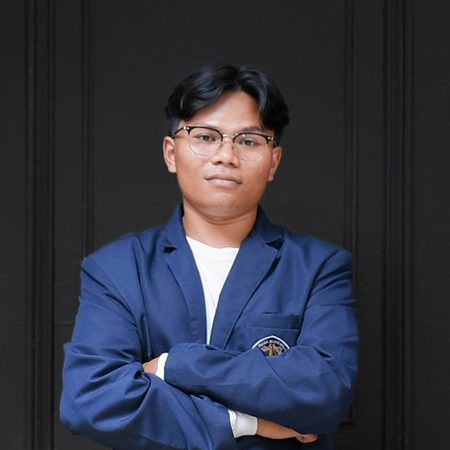
\includegraphics[width=0.82\linewidth,height=3.4cm,keepaspectratio]{public/assets/image/saya.jpg} \par \vspace{3pt}
        {\scriptsize \bfseries \color{brandNavy} Varizky Naldiba Rimra} \par
        {\tiny \color{brandSlate} Politeknik Negeri Malang}
      \end{tcolorbox}
    \end{column}
  \end{columns}
\end{frame}

% ==============================================================================
% SLIDE 04: PENDIDIKAN & 6 PRESTASI TERVERIFIKASI
% ==============================================================================
\begin{frame}{Pendidikan \& 6 Prestasi Terverifikasi}{DOKUMEN RESMI \& KOMPETISI}
  \begin{columns}[t]
    \begin{column}{0.42\textwidth}
      \begin{tcolorbox}[colback=brandCardBg,colframe=brandBorder,arc=2mm,boxrule=0.6pt,boxsep=3pt,top=4pt,bottom=4pt,title={\footnotesize \bfseries \color{brandNavy} Riwayat Akademik}]
        {\small \bfseries \color{brandNavy} D4 Teknik Informatika} \par
        {\scriptsize \bfseries \color{brandBlue} Politeknik Negeri Malang (Polinema)} \par
        {\tiny \color{brandSlate} 2022 -- Sekarang \ $|$ \ IPK Memuaskan} \par \vspace{3pt}
        {\scriptsize \color{brandDark}
        $\bullet$ \textbf{Fokus Studi:} Applied AI, IoT Telemetry, WebGIS \& Sistem Informasi. \\
        $\bullet$ \textbf{Model Pembelajaran:} Project-Based Learning (PBL) dan riset terapan institusional. \\
        $\bullet$ \textbf{Standar Mutu:} Pengujian fungsional ketat, kalibrasi sensor, dan audit trail data.
        }
      \end{tcolorbox}
    \end{column}

    \begin{column}{0.56\textwidth}
      \begin{tcolorbox}[colback=white,colframe=brandBorder,arc=2mm,boxrule=0.6pt,boxsep=2.5pt,top=3pt,bottom=3pt,title={\footnotesize \bfseries \color{brandNavy} 6 Rekam Jejak Prestasi \& Hibah Terverifikasi}]
        {\scriptsize \color{brandDark}
        $\bullet$ \textbf{\color{amberBadgeText}Juara Harapan 2 LKTI Nasional} -- TFS 2026 (SK 27881) \par \vspace{2pt}
        $\bullet$ \textbf{\color{blueBadgeText}Lolos Seleksi Tahap 2 Insentif} -- PKM-GFT POLINEMA 2026 (SK 40) \par \vspace{2pt}
        $\bullet$ \textbf{\color{brandNavy}Peringkat 18 / 82 Tim Nasional} -- Intelecta Cup (Skor: \textbf{94.310}) \par \vspace{2pt}
        $\bullet$ \textbf{\color{brandNavy}Finalis Nasional LKTI} -- TFS 2025 (SK No. 16002/PL2.3/KM/2025) \par \vspace{2pt}
        $\bullet$ \textbf{\color{brandNavy}Peserta Resmi} -- Data Mining Hology 8.0 (Tim Penyelam Handal) \par \vspace{2pt}
        $\bullet$ \textbf{\color{brandNavy}Peserta Resmi} -- Jatim Datathon 2025 (Tim Maju Lancar)
        }
      \end{tcolorbox}
    \end{column}
  \end{columns}
\end{frame}

% ==============================================================================
% SLIDE 05: 4 PILAR KEAHLIAN TEKNIS
% ==============================================================================
\begin{frame}{4 Pilar Keahlian Teknis}{KOMPETENSI HULU-KE-HILIR EDGE HINGGA CLOUD}
  \begin{columns}[t]
    \begin{column}{0.24\textwidth}
      \begin{tcolorbox}[colback=brandCardBg,colframe=brandBorder,arc=2mm,boxrule=0.6pt,boxsep=2pt,top=3pt,bottom=3pt,title={\scriptsize \bfseries \color{brandNavy} 1. AI \& Vision}]
        {\tiny \color{brandDark}
        $\bullet$ \textbf{Framework:} TensorFlow, PyTorch, Scikit-Learn. \\ \vspace{2pt}
        $\bullet$ \textbf{Model:} MCNN, CSRNet, LSTM, SVM. \\ \vspace{2pt}
        $\bullet$ \textbf{Vision:} OpenCV, GLCM, Wavelet 2D, HOG. \\ \vspace{2pt}
        $\bullet$ \textbf{GenAI:} Google Gemini API, Prompt Structured.
        }
      \end{tcolorbox}
    \end{column}

    \begin{column}{0.24\textwidth}
      \begin{tcolorbox}[colback=brandCardBg,colframe=brandBorder,arc=2mm,boxrule=0.6pt,boxsep=2pt,top=3pt,bottom=3pt,title={\scriptsize \bfseries \color{brandNavy} 2. IoT Telemetri}]
        {\tiny \color{brandDark}
        $\bullet$ \textbf{Board:} ESP32, Arduino, Optocoupler Relay. \\ \vspace{2pt}
        $\bullet$ \textbf{Sensor:} pH, Turbidity, DS18B20 Temp, DO. \\ \vspace{2pt}
        $\bullet$ \textbf{Firmware:} Polinomial Curves, Temp Compensate. \\ \vspace{2pt}
        $\bullet$ \textbf{Failover:} Flash Ring Buffer (Zero Loss).
        }
      \end{tcolorbox}
    \end{column}

    \begin{column}{0.24\textwidth}
      \begin{tcolorbox}[colback=brandCardBg,colframe=brandBorder,arc=2mm,boxrule=0.6pt,boxsep=2pt,top=3pt,bottom=3pt,title={\scriptsize \bfseries \color{brandNavy} 3. Geospatial}]
        {\tiny \color{brandDark}
        $\bullet$ \textbf{Mapping:} Leaflet, OpenStreetMap, GeoJSON. \\ \vspace{2pt}
        $\bullet$ \textbf{Spatial:} Disparity Index, Klaster K-Means. \\ \vspace{2pt}
        $\bullet$ \textbf{Integrasi:} Radar BMKG, BPBD, BPS. \\ \vspace{2pt}
        $\bullet$ \textbf{ETL:} Levenshtein Fuzzy Matching Wilayah.
        }
      \end{tcolorbox}
    \end{column}

    \begin{column}{0.24\textwidth}
      \begin{tcolorbox}[colback=brandCardBg,colframe=brandBorder,arc=2mm,boxrule=0.6pt,boxsep=2pt,top=3pt,bottom=3pt,title={\scriptsize \bfseries \color{brandNavy} 4. Full-Stack}]
        {\tiny \color{brandDark}
        $\bullet$ \textbf{Web:} React, Next.js, Laravel, Streamlit. \\ \vspace{2pt}
        $\bullet$ \textbf{Database:} Firebase DB, MySQL ACID. \\ \vspace{2pt}
        $\bullet$ \textbf{SPK:} PROMETHEE DSS, BCG Menu Matrix. \\ \vspace{2pt}
        $\bullet$ \textbf{DevOps:} Git, GitHub, HuggingFace, Linux.
        }
      \end{tcolorbox}
    \end{column}
  \end{columns}
\end{frame}

% ==============================================================================
% SLIDE 06: MATRIKS TAKSONOMI 13 PROYEK
% ==============================================================================
\begin{frame}{Matriks Taksonomi 13 Proyek}{TAKSONOMI 13 PROYEK}
  \begin{columns}[t]
    \begin{column}{0.24\textwidth}
      \begin{tcolorbox}[colback=brandCardBg,colframe=brandBorder,arc=2mm,boxrule=0.6pt,boxsep=2pt,top=3pt,bottom=3pt,title={\scriptsize \bfseries \color{brandNavy} A. Akuakultur IoT}]
        {\tiny \color{brandDark}
        $\bullet$ \textbf{01. Aquavion:} Telemetri Tambak Lele (Next.js) \\ \vspace{2pt}
        $\bullet$ \textbf{02. CatfishCare:} Aerasi Otomatis (\textbf{Harapan 2}) \\ \vspace{2pt}
        $\bullet$ \textbf{03. SAIS:} Smart Fishfarm (\textbf{PKM-GFT}) \\ \vspace{2pt}
        $\bullet$ \textbf{05. AlgaSense:} Rumput Laut (\textbf{Finalis TFS})
        }
      \end{tcolorbox}
    \end{column}

    \begin{column}{0.24\textwidth}
      \begin{tcolorbox}[colback=brandCardBg,colframe=brandBorder,arc=2mm,boxrule=0.6pt,boxsep=2pt,top=3pt,bottom=3pt,title={\scriptsize \bfseries \color{brandNavy} B. AI \& Machine Learning}]
        {\tiny \color{brandDark}
        $\bullet$ \textbf{06. Crowd Density:} MCNN Hology 8.0 \\ \vspace{2pt}
        $\bullet$ \textbf{07. Agroclimatology:} Cuaca (\textbf{Rank 18 / 82}) \\ \vspace{2pt}
        $\bullet$ \textbf{09. AI Restaurant:} Gemini API \& BCG \\ \vspace{2pt}
        $\bullet$ \textbf{10. Fruit Classifier:} GLCM/HOG + SVM
        }
      \end{tcolorbox}
    \end{column}

    \begin{column}{0.24\textwidth}
      \begin{tcolorbox}[colback=brandCardBg,colframe=brandBorder,arc=2mm,boxrule=0.6pt,boxsep=2pt,top=3pt,bottom=3pt,title={\scriptsize \bfseries \color{brandNavy} C. Geospasial \& GIS}]
        {\tiny \color{brandDark}
        $\bullet$ \textbf{04. Si Mojang:} Riset Terapan BRIN Banjir \\ \vspace{2pt}
        $\bullet$ \textbf{08. SLB Disparity:} Datathon Jatim 2025 \\ \vspace{2pt}
        $\bullet$ \textbf{13. School GIS:} Klaster Sekolah K-Means
        }
      \end{tcolorbox}
    \end{column}

    \begin{column}{0.24\textwidth}
      \begin{tcolorbox}[colback=brandCardBg,colframe=brandBorder,arc=2mm,boxrule=0.6pt,boxsep=2pt,top=3pt,bottom=3pt,title={\scriptsize \bfseries \color{brandNavy} D. Enterprise \& SPK}]
        {\tiny \color{brandDark}
        $\bullet$ \textbf{11. SIMPRES:} Portal Prestasi TI + PROMETHEE DSS \\ \vspace{2pt}
        $\bullet$ \textbf{12. Tata Tertib:} Disiplin Mahasiswa Polinema
        }
      \end{tcolorbox}
    \end{column}
  \end{columns}
\end{frame}

% ==============================================================================
% SLIDE 07: PROYEK 01 - AQUAVION
% ==============================================================================
\begin{frame}{P01: Aquavion}{IOT FRESHWATER AQUACULTURE TELEMETRY}
  \begin{columns}[c]
    \begin{column}{0.48\textwidth}
      \begin{tcolorbox}[colback=white,colframe=brandBorder,arc=2mm,boxrule=0.6pt,boxsep=1pt,top=2pt,bottom=2pt,halign=center]
        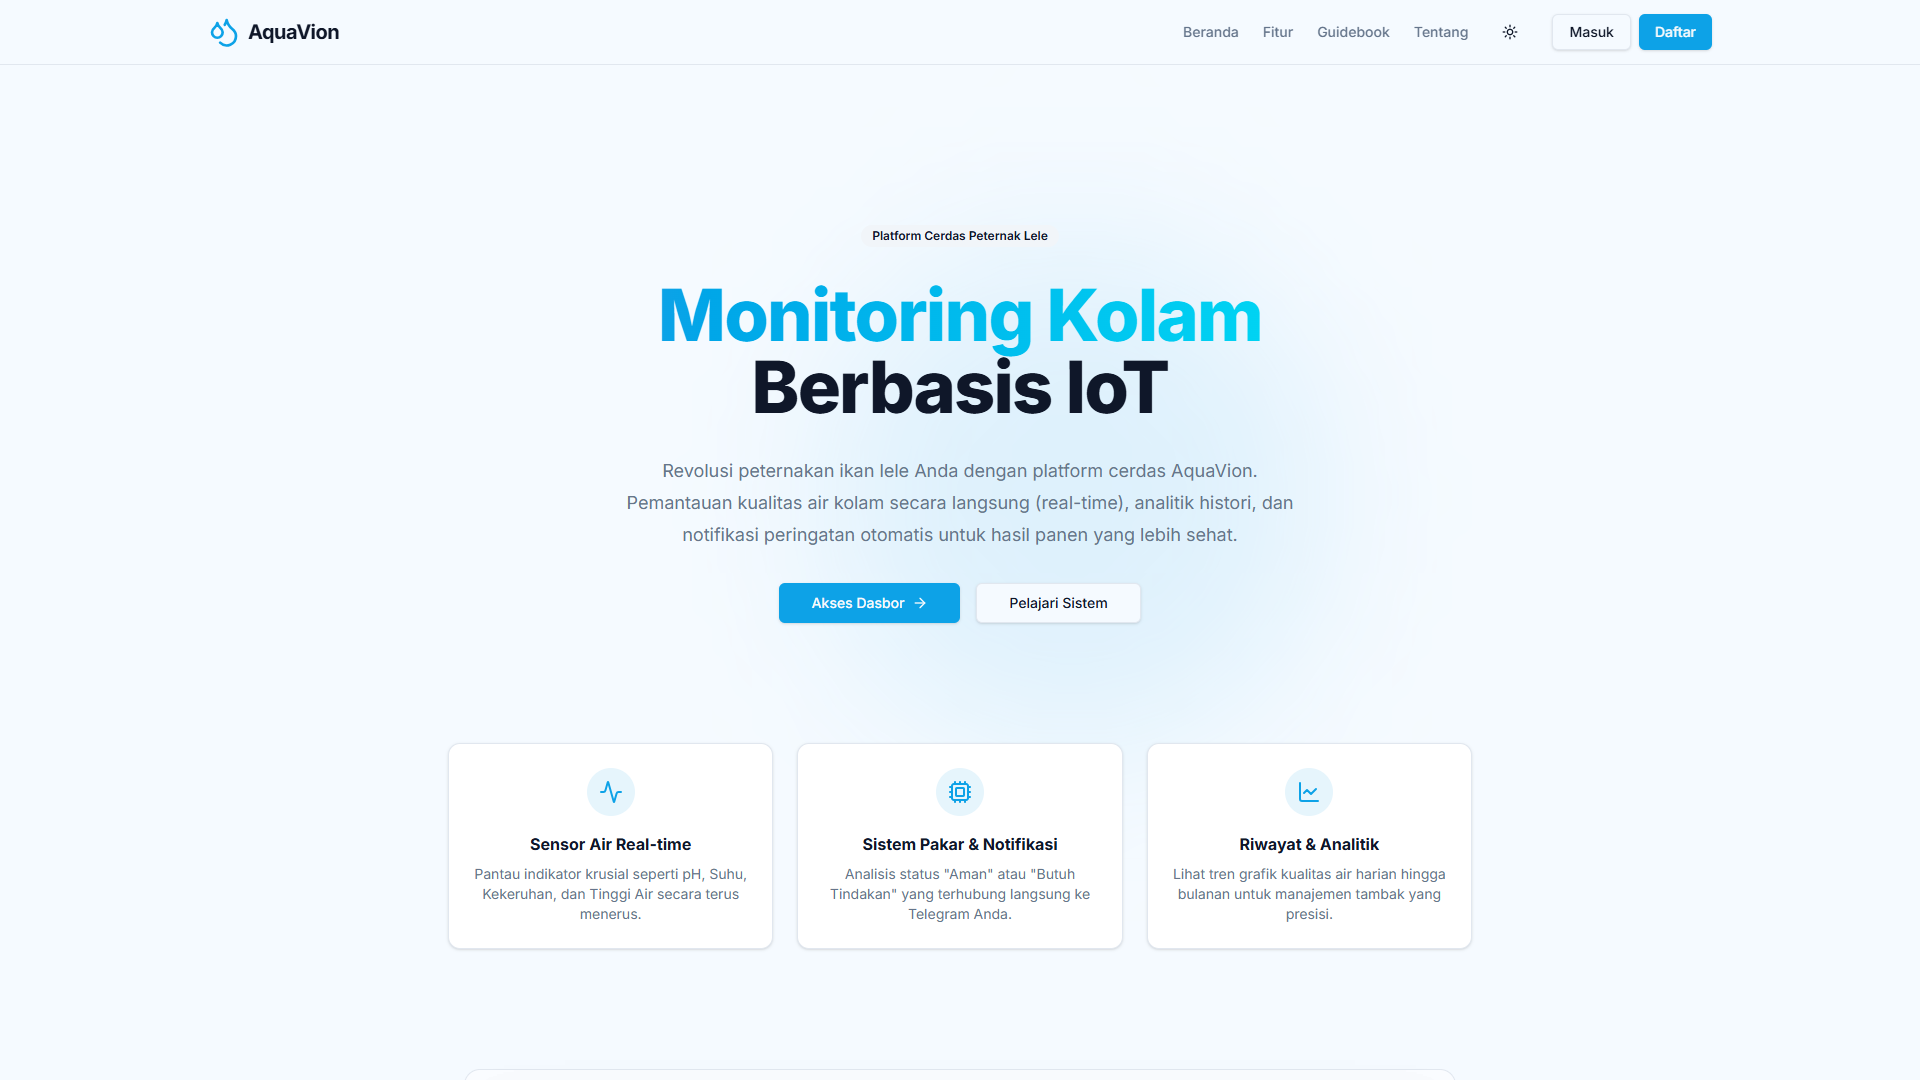
\includegraphics[width=\linewidth,height=3.6cm,keepaspectratio]{src/projects/01-aquavion/assets/aquavion-dashboard-live.png}
      \end{tcolorbox}
      \vspace{2pt}
      \centering
      {\scriptsize \href{https://aqua-vion.vercel.app/}{\color{brandBlue}\textbf{\underline{[Live App: aqua-vion.vercel.app $\nearrow$]}}}}
    \end{column}
    \begin{column}{0.50\textwidth}
      {\scriptsize \color{brandBlue} \textbf{IOT TELEMETRY \& WEB DASHBOARD}} \hfill {\tiny \color{brandSlate} Proyek 01 / 13} \par \vspace{1pt}
      {\large \bfseries \color{brandNavy} Aquavion} \par
      {\scriptsize \bfseries \color{brandDark} Peran: Systems Lead \& IoT Firmware Engineer} \par
      {\tiny \color{brandSlate} \textbf{Tech Stack:} Next.js, Firebase Realtime DB, ESP32, C++, Sensor Probes} \par \vspace{4pt}
      
      {\scriptsize \color{brandDark}
      $\bullet$ \textbf{Telemetri Kolam Multi-Sensor:} Monitoring pH, kekeruhan nephelometric, dan suhu DS18B20 seketika untuk mencegah kematian massal ikan lele. \\
      $\bullet$ \textbf{Kalibrasi Non-Linear:} Menanamkan kurva kalibrasi polinomial dan kompensasi temperatur suhu seketika pada firmware ESP32. \\
      $\bullet$ \textbf{Failover Buffer Sirkular 0\% Loss:} Caching pembacaan sensor pada flash memory lokal saat koneksi internet offline, auto-sinkronisasi pasca rekoneksi.
      }
    \end{column}
  \end{columns}
\end{frame}

% ==============================================================================
% SLIDE 08: PROYEK 02 - CATFISHCARE
% ==============================================================================
\begin{frame}{P02: CatfishCare}{JUARA HARAPAN 2 LKTI TFS 2026}
  \begin{columns}[c]
    \begin{column}{0.48\textwidth}
      \begin{tcolorbox}[colback=white,colframe=brandBorder,arc=2mm,boxrule=0.6pt,boxsep=1pt,top=2pt,bottom=2pt,halign=center]
        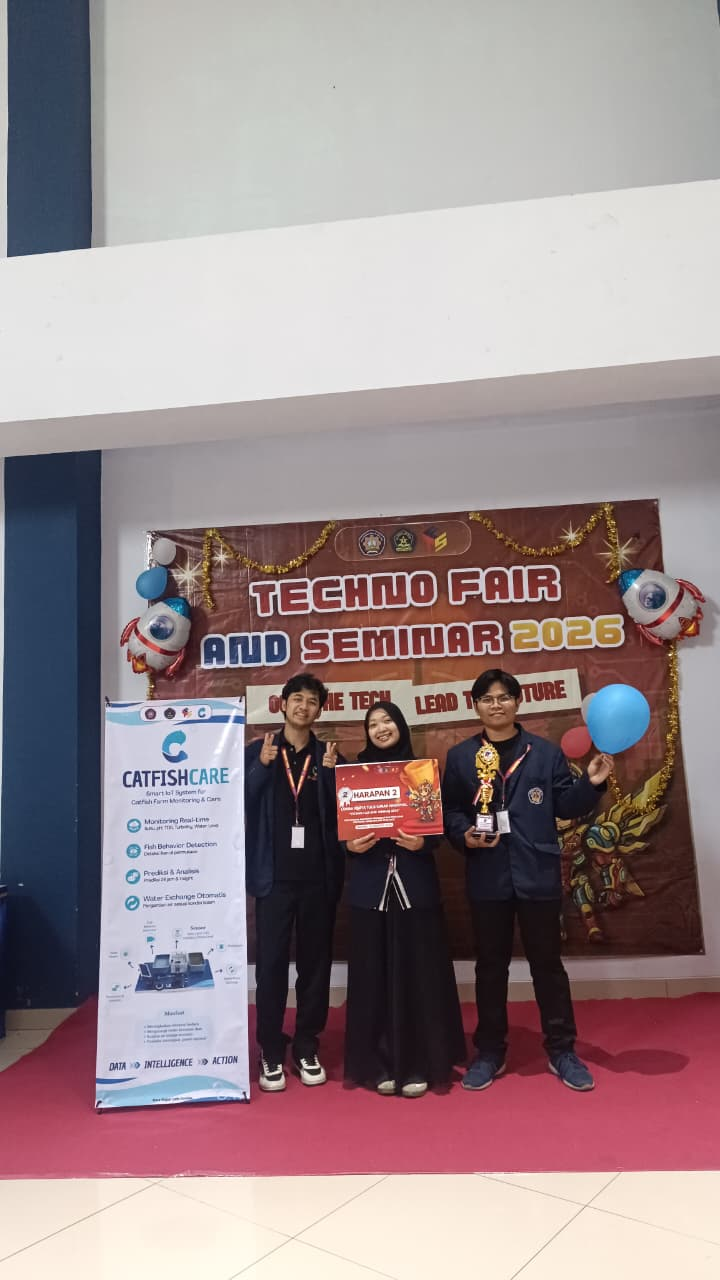
\includegraphics[width=\linewidth,height=3.6cm,keepaspectratio]{src/projects/02-catfishcare-tfs2026/assets/piala-juara-harapan-2.jpg}
      \end{tcolorbox}
      \vspace{2pt}
      \centering
      {\scriptsize \href{https://github.com/VarizkyNaldiba/Smart_Aqua_IOT}{\color{brandBlue}\textbf{\underline{[GitHub: Smart\_Aqua\_IOT $\nearrow$]}}}}
    \end{column}
    \begin{column}{0.50\textwidth}
      {\scriptsize \color{amberBadgeText} \textbf{JUARA HARAPAN 2 LKTI NASIONAL TFS 2026}} \hfill {\tiny \color{brandSlate} Proyek 02 / 13} \par \vspace{1pt}
      {\large \bfseries \color{brandNavy} CatfishCare} \par
      {\scriptsize \bfseries \color{brandDark} Peran: Lead Systems Architect \& Competitor} \par
      {\tiny \color{brandSlate} \textbf{Tech Stack:} ESP32, C++, Closed-Loop Aeration, Relay Optocoupler, Probes} \par \vspace{4pt}
      
      {\scriptsize \color{brandDark}
      $\bullet$ \textbf{Penghargaan Ilmiah Nasional:} Meraih Juara Harapan 2 LKTI Nasional pada Techno Fair and Seminar (TFS) 2026 Polinema (SK No. 27881/PL2.3/KM/2026). \\
      $\bullet$ \textbf{Aktuasi Otomatis Closed-Loop:} Kontrol otomatis pompa aerasi dan sirkulasi air berdasarkan ambang batas oksigen terlarut dan pH secara real-time. \\
      $\bullet$ \textbf{Isolasi Galvanik Perangkat:} Menerapkan relay optocoupler untuk mengisolasi logika kontroler dari derau lonjakan induktif motor pompa kolam.
      }
    \end{column}
  \end{columns}
\end{frame}

% ==============================================================================
% SLIDE 09: PROYEK 03 - SAIS
% ==============================================================================
\begin{frame}{P03: SAIS}{HIBAH RISET PKM-GFT POLINEMA 2026 TAHAP 2}
  \begin{columns}[c]
    \begin{column}{0.48\textwidth}
      \begin{tcolorbox}[colback=white,colframe=brandBorder,arc=2mm,boxrule=0.6pt,boxsep=1pt,top=2pt,bottom=2pt,halign=center]
        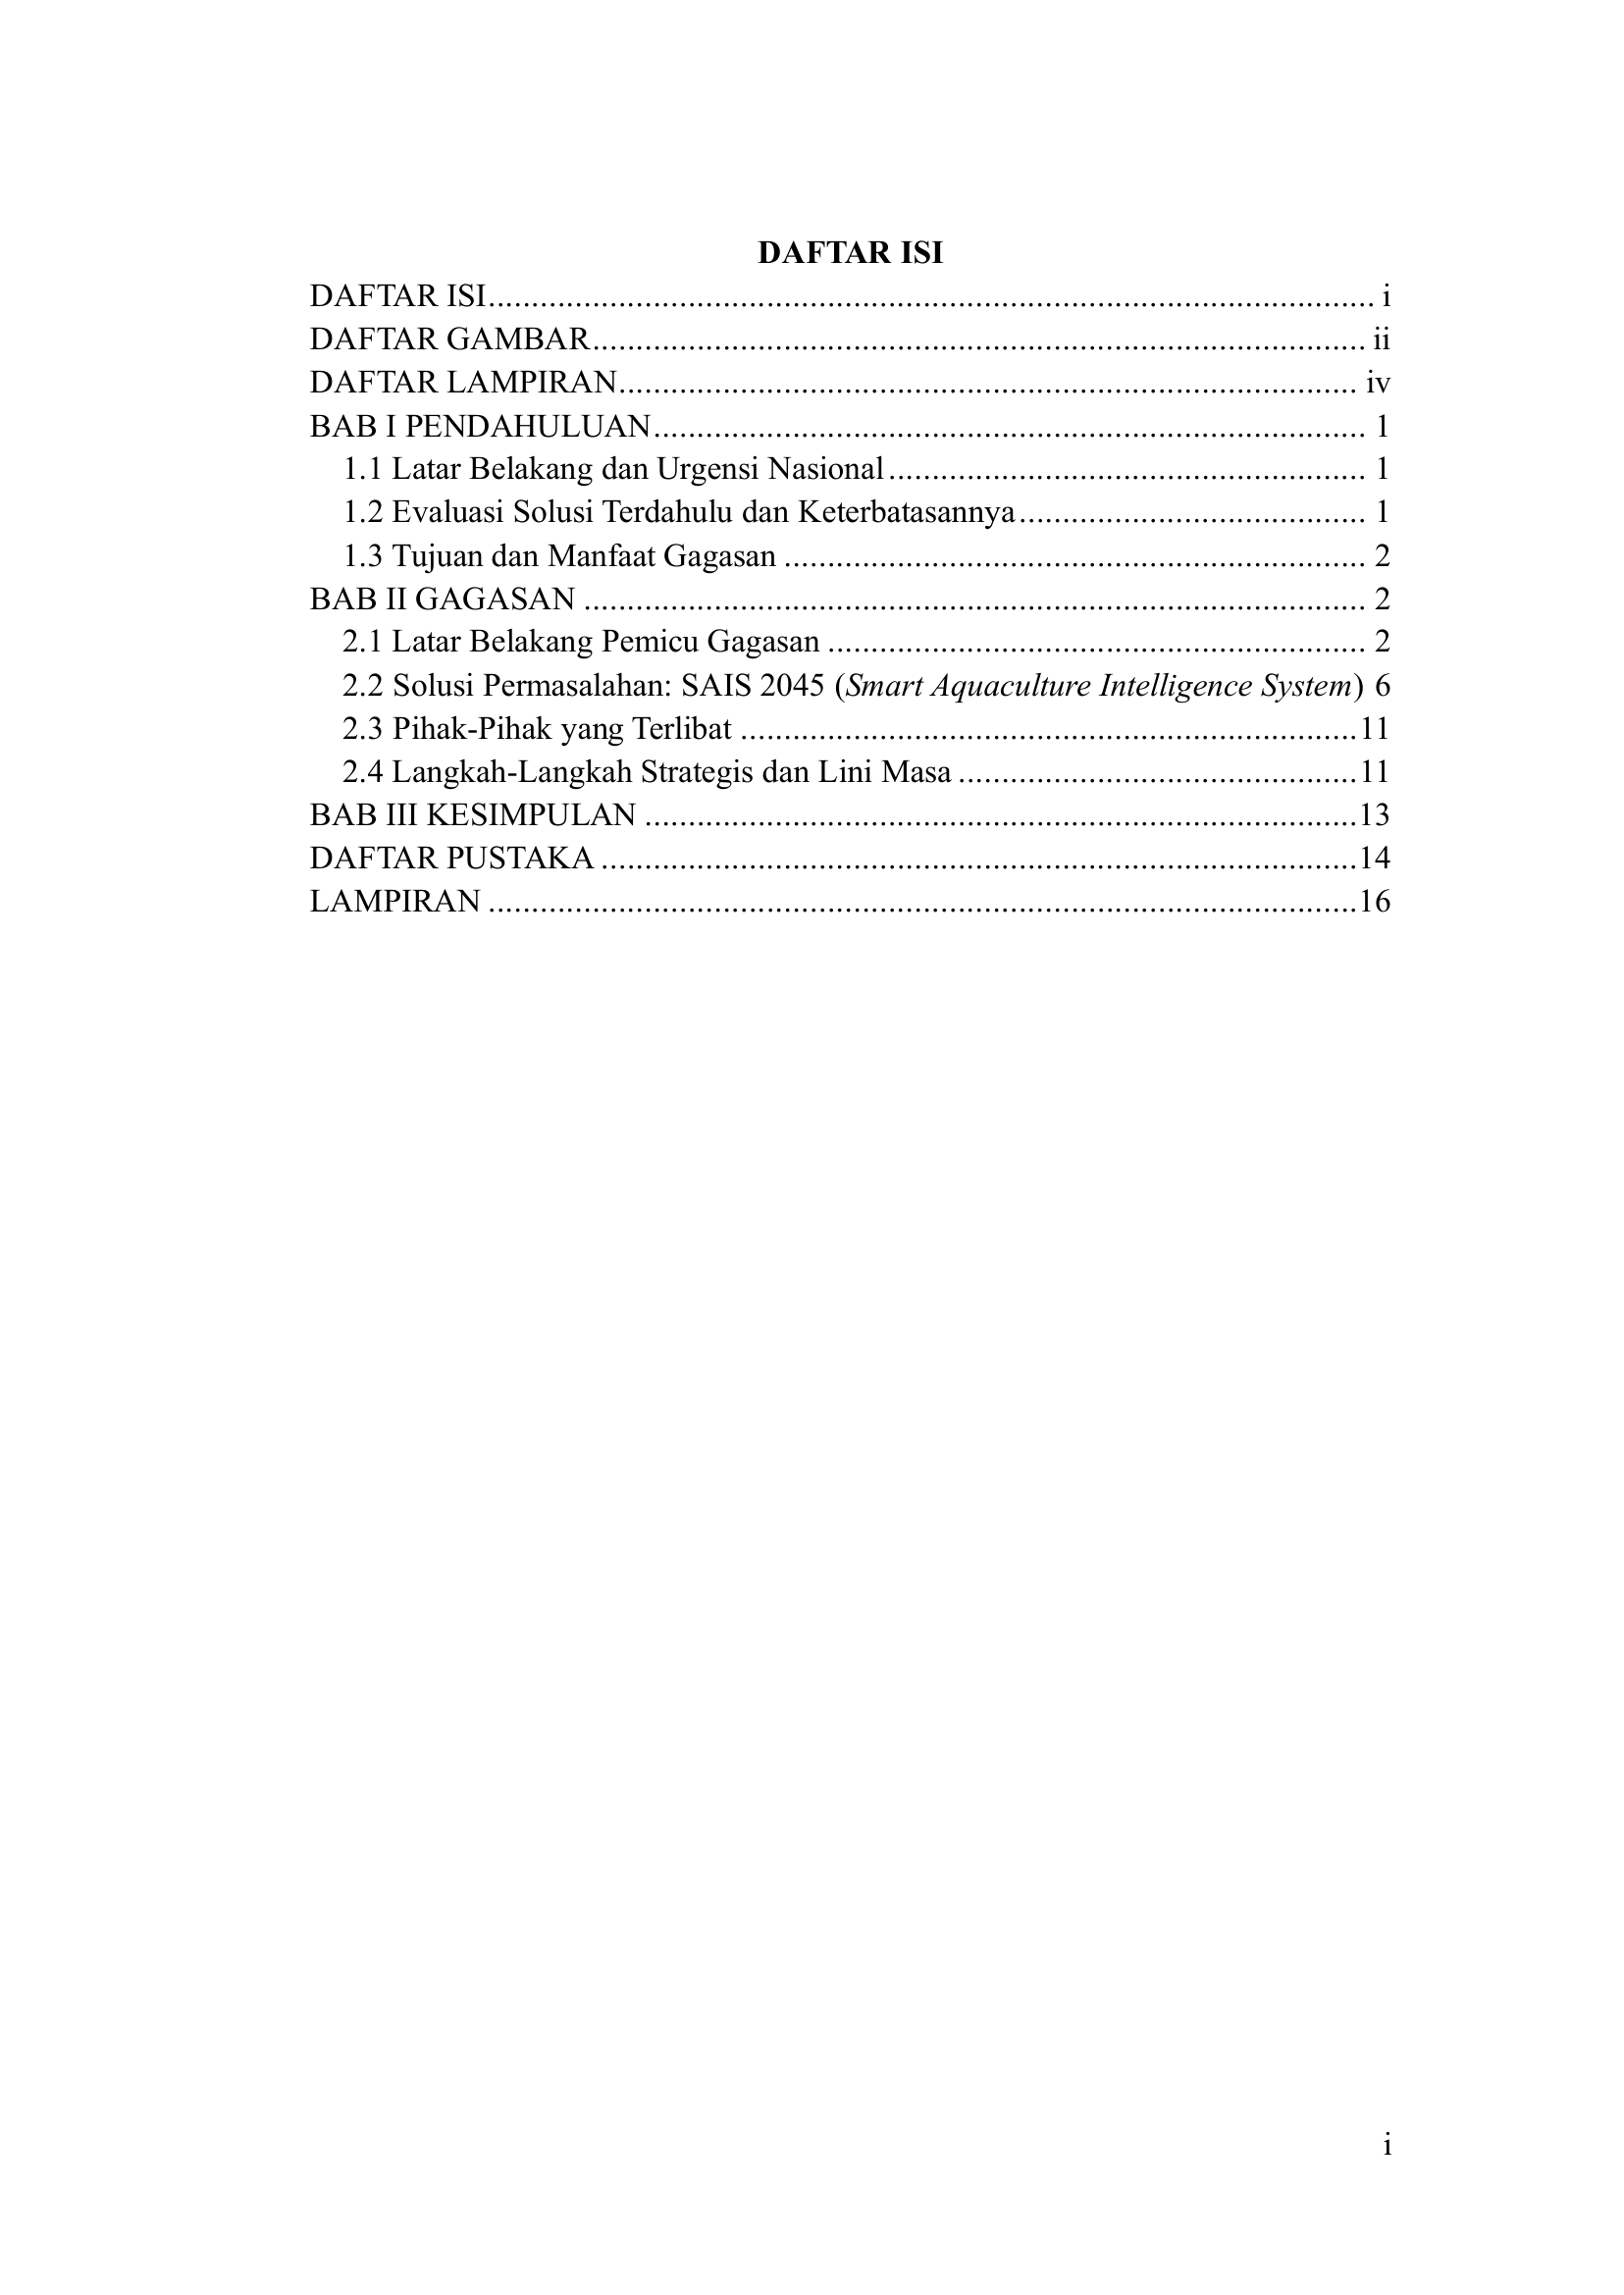
\includegraphics[width=\linewidth,height=3.6cm,keepaspectratio]{src/projects/03-pkm-gft-sais/assets/proposal-sais-pkm-gft.png}
      \end{tcolorbox}
      \vspace{2pt}
      \centering
      {\scriptsize \color{brandSlate} \textbf{[SK Insentif No. 40/WADIR.III/KM/2026]}}
    \end{column}
    \begin{column}{0.50\textwidth}
      {\scriptsize \color{blueBadgeText} \textbf{LOLOS SELEKSI TAHAP 2 INSENTIF PKM 2026}} \hfill {\tiny \color{brandSlate} Proyek 03 / 13} \par \vspace{1pt}
      {\large \bfseries \color{brandNavy} Smart Aquaculture Intelligence} \par
      {\scriptsize \bfseries \color{brandDark} Peran: Principal Author \& System Conceptor} \par
      {\tiny \color{brandSlate} \textbf{Tech Stack:} AI Systems, Digital Twin Modeling, Autonomous IoT Network} \par \vspace{4pt}
      
      {\scriptsize \color{brandDark}
      $\bullet$ \textbf{Blueprint Ketahanan Pangan 2045:} Gagasan futuristik tertulis mentransformasikan tambak konvensional menjadi ekosistem akuakultur pintar terdistribusi. \\
      $\bullet$ \textbf{Pemodelan Digital Twin:} Simulasi parameter fisika-kimia air kolam dan estimasi dinamika biomassa ikan berbasis model komputasi prediktif. \\
      $\bullet$ \textbf{Arsitektur Tiga Tingkat:} Pemisahan tegas loop penyelamatan cepat di edge dan analitik agregat regional di level cloud.
      }
    \end{column}
  \end{columns}
\end{frame}

% ==============================================================================
% SLIDE 10: PROYEK 04 - SI MOJANG BRANTAS
% ==============================================================================
\begin{frame}{P04: Si Mojang Brantas}{WEBGIS MONITORING BANJIR RISET TERAPAN BRIN}
  \begin{columns}[c]
    \begin{column}{0.48\textwidth}
      \begin{tcolorbox}[colback=white,colframe=brandBorder,arc=2mm,boxrule=0.6pt,boxsep=1pt,top=2pt,bottom=2pt,halign=center]
        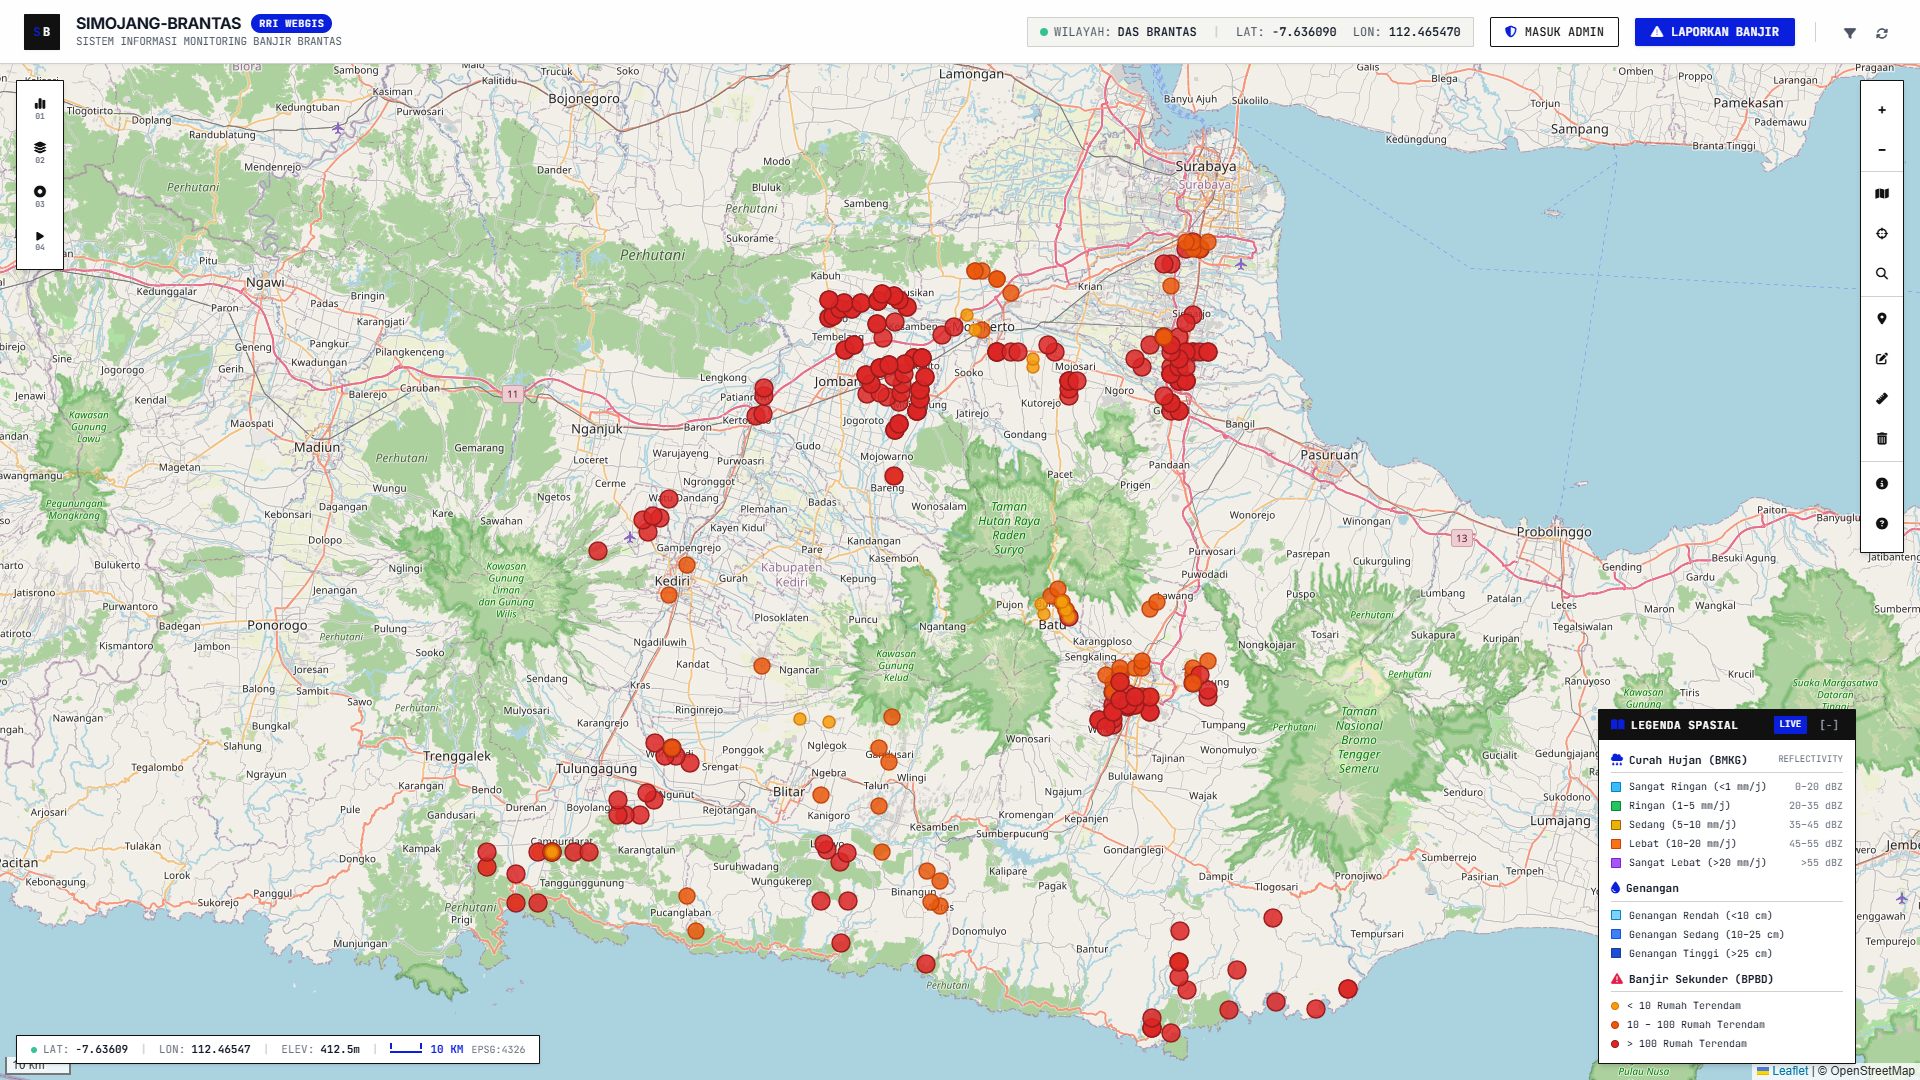
\includegraphics[width=\linewidth,height=3.6cm,keepaspectratio]{src/projects/04-simojang-brin-webgis/assets/simojang-live-map.png}
      \end{tcolorbox}
      \vspace{2pt}
      \centering
      {\scriptsize \href{https://simojang.let.polinema.ac.id/}{\color{brandBlue}\textbf{\underline{[Live: simojang.let.polinema.ac.id $\nearrow$]}}}}
    \end{column}
    \begin{column}{0.50\textwidth}
      {\scriptsize \color{brandBlue} \textbf{RISET TERAPAN BRIN X POLINEMA}} \hfill {\tiny \color{brandSlate} Proyek 04 / 13} \par \vspace{1pt}
      {\large \bfseries \color{brandNavy} Si Mojang Brantas} \par
      {\scriptsize \bfseries \color{brandDark} Peran: IT \& WebGIS Production Developer} \par
      {\tiny \color{brandSlate} \textbf{Tech Stack:} Leaflet, GeoJSON, OpenStreetMap, Telemetri Radar BMKG, Spatial DB} \par \vspace{4pt}
      
      {\scriptsize \color{brandDark}
      $\bullet$ \textbf{Platform WebGIS Produksi Aktif:} Beroperasi penuh pada domain resmi \href{https://simojang.let.polinema.ac.id/}{\color{brandBlue}\underline{simojang.let.polinema.ac.id}} untuk mitigasi banjir DAS Brantas Hulu. \\
      $\bullet$ \textbf{Integrasi Multidata Spasial:} Menyatukan peta kontur elevasi, batas administrasi, radar reflektivitas hujan BMKG, dan data genangan BPBD. \\
      $\bullet$ \textbf{Pelaporan Warga Partisipatif:} Pintu masuk masyarakat melaporkan tinggi muka air banjir secara real-time dengan validasi geofencing GPS.
      }
    \end{column}
  \end{columns}
\end{frame}

% ==============================================================================
% SLIDE 11: PROYEK 05 - ALGASENSE
% ==============================================================================
\begin{frame}{P05: AlgaSense}{TELEMETRI OSEANOGRAFI TFS 2025}
  \begin{columns}[c]
    \begin{column}{0.48\textwidth}
      \begin{tcolorbox}[colback=white,colframe=brandBorder,arc=2mm,boxrule=0.6pt,boxsep=1pt,top=2pt,bottom=2pt,halign=center]
        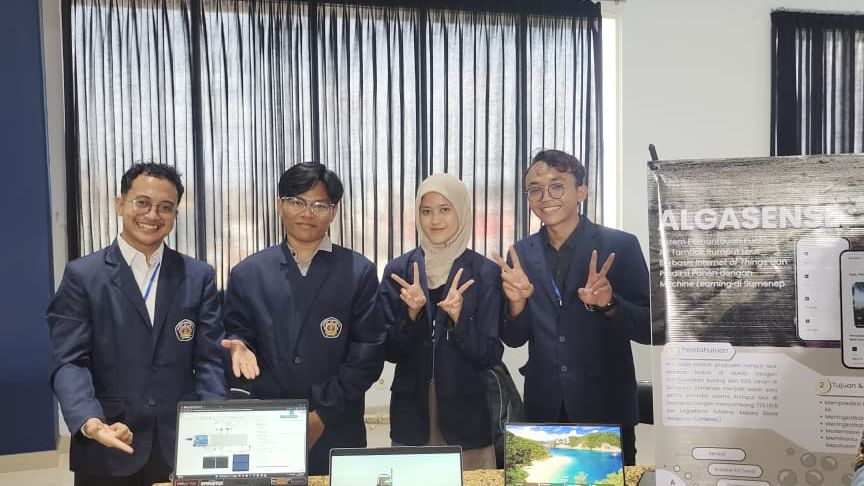
\includegraphics[width=\linewidth,height=3.6cm,keepaspectratio]{src/projects/05-algasense/assets/tim-algasense-banner.jpg}
      \end{tcolorbox}
      \vspace{2pt}
      \centering
      {\scriptsize \href{https://github.com/VarizkyNaldiba/Algasense}{\color{brandBlue}\textbf{\underline{[GitHub: Algasense $\nearrow$]}}}}
    \end{column}
    \begin{column}{0.50\textwidth}
      {\scriptsize \color{amberBadgeText} \textbf{FINALIS NASIONAL LKTI TFS 2025}} \hfill {\tiny \color{brandSlate} Proyek 05 / 13} \par \vspace{1pt}
      {\large \bfseries \color{brandNavy} AlgaSense: Marine IoT \& ML} \par
      {\scriptsize \bfseries \color{brandDark} Peran: Machine Learning \& Embedded Systems Engineer} \par
      {\tiny \color{brandSlate} \textbf{Tech Stack:} Python, TensorFlow, Keras LSTM, ESP32, Sensor Salinitas \& DO} \par \vspace{4pt}
      
      {\scriptsize \color{brandDark}
      $\bullet$ \textbf{Inovasi Kelautan Terverifikasi:} Lolos sebagai Finalis Nasional LKTI TFS 2025 (SK No. 16002/PL2.3/KM/2025) di pesisir Sumenep, Madura. \\
      $\bullet$ \textbf{Prediksi Deret Waktu LSTM:} Model rekuren LSTM memproses dinamika salinitas air laut, oksigen terlarut, dan suhu untuk estimasi kurva panen. \\
      $\bullet$ \textbf{Instrumen Tahan Korosi Air Asin:} Pengondisian sinyal analog probe bawah laut terlindung terhadap turbulensi gelombang pesisir.
      }
    \end{column}
  \end{columns}
\end{frame}

% ==============================================================================
% SLIDE 12: PROYEK 06 - CROWD DENSITY ESTIMATION
% ==============================================================================
\begin{frame}{P06: Crowd Density Estimation}{MULTI-COLUMN CNN HOLOGY 8.0}
  \begin{columns}[c]
    \begin{column}{0.48\textwidth}
      \begin{tcolorbox}[colback=white,colframe=brandBorder,arc=2mm,boxrule=0.6pt,boxsep=1pt,top=2pt,bottom=2pt,halign=center]
        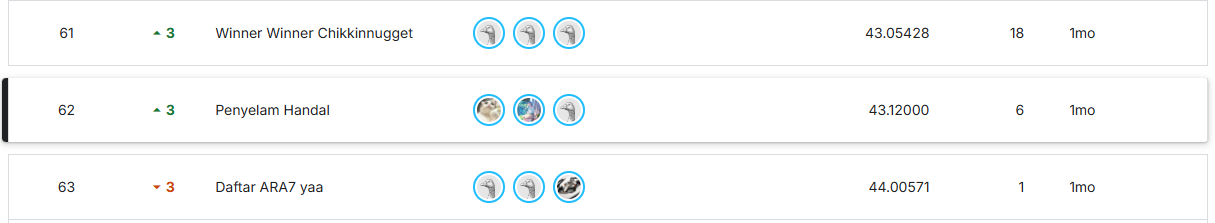
\includegraphics[width=\linewidth,height=3.6cm,keepaspectratio]{src/projects/06-crowd-density-hology/assets/hology-density-model.png}
      \end{tcolorbox}
      \vspace{2pt}
      \centering
      {\scriptsize \href{https://github.com/VarizkyNaldiba/PenyelamHandal_Hology}{\color{brandBlue}\textbf{\underline{[GitHub: PenyelamHandal\_Hology $\nearrow$]}}}}
    \end{column}
    \begin{column}{0.50\textwidth}
      {\scriptsize \color{brandBlue} \textbf{PESERTA RESMI DATA MINING HOLOGY 8.0}} \hfill {\tiny \color{brandSlate} Proyek 06 / 13} \par \vspace{1pt}
      {\large \bfseries \color{brandNavy} Crowd Density Estimation} \par
      {\scriptsize \bfseries \color{brandDark} Peran: Deep Learning Researcher (Tim Penyelam Handal)} \par
      {\tiny \color{brandSlate} \textbf{Tech Stack:} Python, PyTorch, TensorFlow, MCNN, CSRNet, OpenCV} \par \vspace{4pt}
      
      {\scriptsize \color{brandDark}
      $\bullet$ \textbf{Kompetisi Nasional Hology 8.0:} Membangun model estimasi kepadatan massa pada citra pengawasan resolusi tinggi tanpa batas terkendali. \\
      $\bullet$ \textbf{Multi-Column CNN (MCNN):} Tiga cabang konvolusi paralel ($3\times3$, $5\times5$, $7\times7$) menangkap variasi skala kepala akibat distorsi perspektif kamera. \\
      $\bullet$ \textbf{Peta Kepadatan Gaussian:} Transformasi anotasi titik koordinat kepala menjadi peta densitas kontinu berlandaskan sebaran kernel Gaussian.
      }
    \end{column}
  \end{columns}
\end{frame}

% ==============================================================================
% SLIDE 13: PROYEK 07 - AGROCLIMATOLOGY
% ==============================================================================
\begin{frame}{P07: Agroclimatology Prediction}{INTELECTA CUP RANK 18 / 82}
  \begin{columns}[c]
    \begin{column}{0.48\textwidth}
      \begin{tcolorbox}[colback=white,colframe=brandBorder,arc=2mm,boxrule=0.6pt,boxsep=1pt,top=2pt,bottom=2pt,halign=center]
        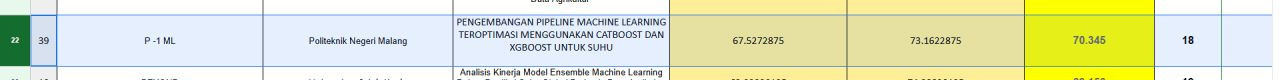
\includegraphics[width=\linewidth,height=3.6cm,keepaspectratio]{src/projects/07-agroclimatology-intelecta/assets/leaderboard-rank18.jpg}
      \end{tcolorbox}
      \vspace{2pt}
      \centering
      {\scriptsize \href{https://github.com/VarizkyNaldiba/Intelecta_P-1ML}{\color{brandBlue}\textbf{\underline{[GitHub: Intelecta\_P-1ML $\nearrow$]}}}}
    \end{column}
    \begin{column}{0.50\textwidth}
      {\scriptsize \color{amberBadgeText} \textbf{PERINGKAT 18 / 82 KAGGLE \ $|$ \ SKOR: 94.310}} \hfill {\tiny \color{brandSlate} Proyek 07 / 13} \par \vspace{1pt}
      {\large \bfseries \color{brandNavy} Agroclimatology Prediction} \par
      {\scriptsize \bfseries \color{brandDark} Peran: ML Engineer \& Data Scientist (Tim P-1 ML)} \par
      {\tiny \color{brandSlate} \textbf{Tech Stack:} Python, CatBoost, XGBoost, Scikit-Learn, Pandas, Feature Engineering} \par \vspace{4pt}
      
      {\scriptsize \color{brandDark}
      $\bullet$ \textbf{Kompetisi Nasional Intelecta Cup 2025:} Memprediksi anomali cuaca dan curah hujan pertanian dengan skor leaderboard resmi 94.310. \\
      $\bullet$ \textbf{Rekayasa Fitur Siklikal:} Transformasi data tanggal ke dalam encoding harmonik sinus/kosinus serta pembuatan fitur lag temperatur multi-periode. \\
      $\bullet$ \textbf{Ensemble Model Gradient Boosting:} Kombinasi regresi CatBoost dan XGBoost dengan validasi silang ketat mencegah overfitting.
      }
    \end{column}
  \end{columns}
\end{frame}

% ==============================================================================
% SLIDE 14: PROYEK 08 - SLB SPATIAL DISPARITY
% ==============================================================================
\begin{frame}{P08: SLB Spatial Disparity Analysis}{JATIM DATATHON 2025}
  \begin{columns}[c]
    \begin{column}{0.48\textwidth}
      \begin{tcolorbox}[colback=white,colframe=brandBorder,arc=2mm,boxrule=0.6pt,boxsep=1pt,top=2pt,bottom=2pt,halign=center]
        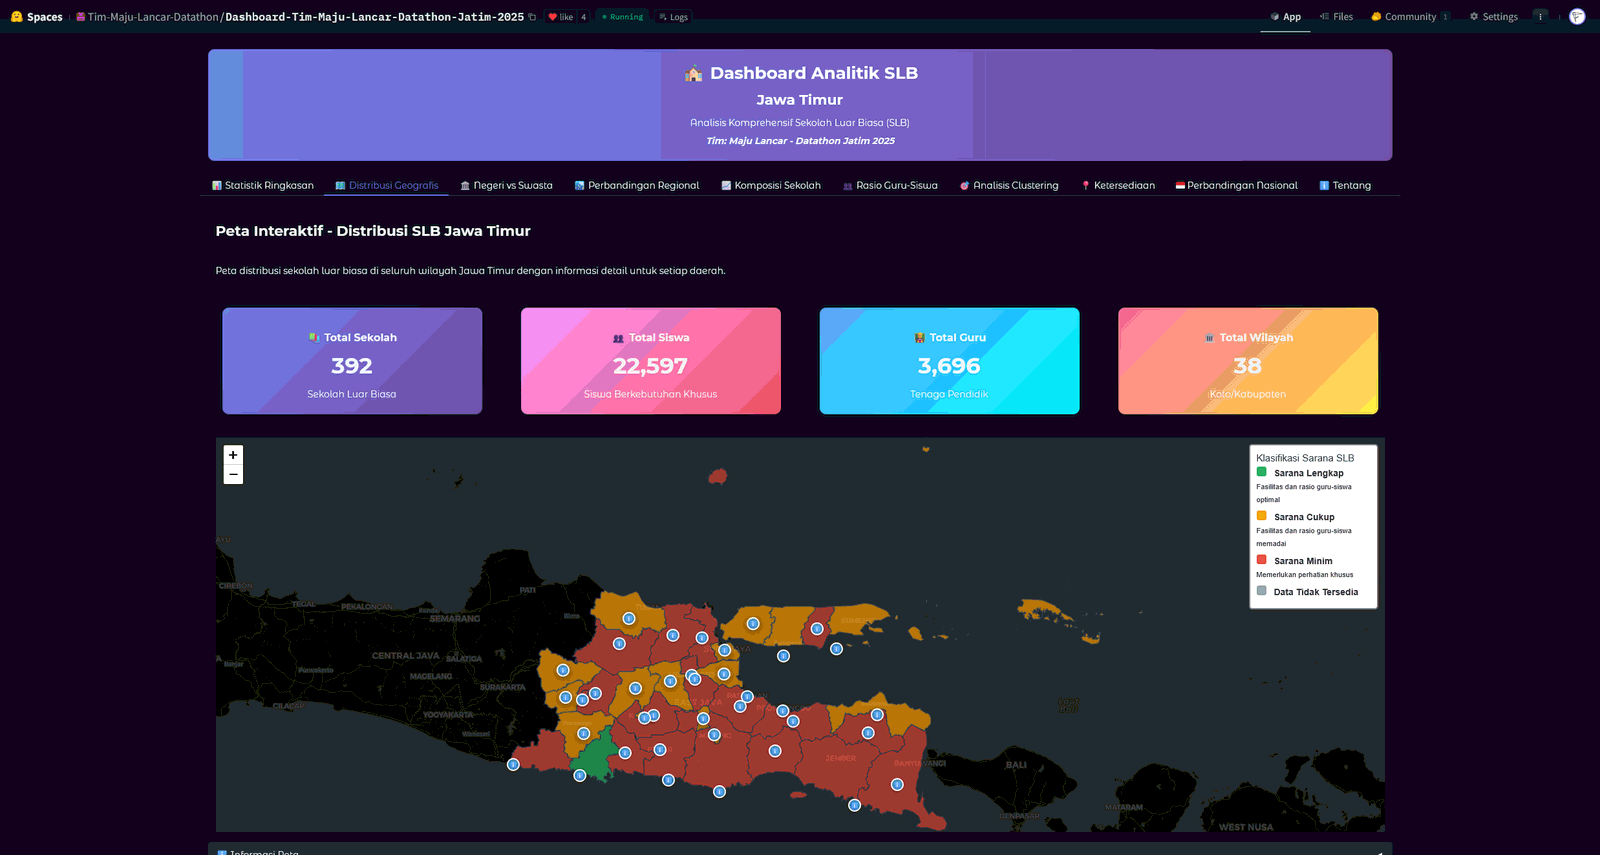
\includegraphics[width=\linewidth,height=3.6cm,keepaspectratio]{src/projects/08-slb-spatial-disparity/assets/datathon1.png}
      \end{tcolorbox}
      \vspace{2pt}
      \centering
      {\scriptsize \href{https://huggingface.co/spaces/Tim-Maju-Lancar-Datathon/Dashboard-Tim-Maju-Lancar-Datathon-Jatim-2025}{\color{brandBlue}\textbf{\underline{[HuggingFace: Dashboard Datathon $\nearrow$]}}}}
    \end{column}
    \begin{column}{0.50\textwidth}
      {\scriptsize \color{brandBlue} \textbf{PESERTA RESMI JATIM DATATHON 2025}} \hfill {\tiny \color{brandSlate} Proyek 08 / 13} \par \vspace{1pt}
      {\large \bfseries \color{brandNavy} SLB Spatial Disparity} \par
      {\scriptsize \bfseries \color{brandDark} Peran: Lead Geospatial Data Analyst (Tim Maju Lancar)} \par
      {\tiny \color{brandSlate} \textbf{Tech Stack:} Python, Pandas, GeoJSON, Folium, Levenshtein Fuzzy, HuggingFace} \par \vspace{4pt}
      
      {\scriptsize \color{brandDark}
      $\bullet$ \textbf{Harmonisasi Data 38 Kab/Kota:} Mengolah data demografi anak berkebutuhan khusus dan sebaran SLB di seluruh Jawa Timur (Diskominfo Prov. Jatim). \\
      $\bullet$ \textbf{Spatial Accessibility Index:} Perumusan rasio kesenjangan daya tampung pendidikan khusus untuk rekomendasi alokasi anggaran pemerintah. \\
      $\bullet$ \textbf{ETL Fuzzy Matching:} Rekonsiliasi data administratif antardinas yang tidak konsisten ke dalam poligon batas wilayah resmi GeoJSON.
      }
    \end{column}
  \end{columns}
\end{frame}

% ==============================================================================
% SLIDE 15: PROYEK 09 - AI RESTAURANT ADVISORY
% ==============================================================================
\begin{frame}{P09: AI Restaurant Advisory System}{SPK KULINER GEMINI API}
  \begin{columns}[c]
    \begin{column}{0.48\textwidth}
      \begin{tcolorbox}[colback=white,colframe=brandBorder,arc=2mm,boxrule=0.6pt,boxsep=1pt,top=2pt,bottom=2pt,halign=center]
        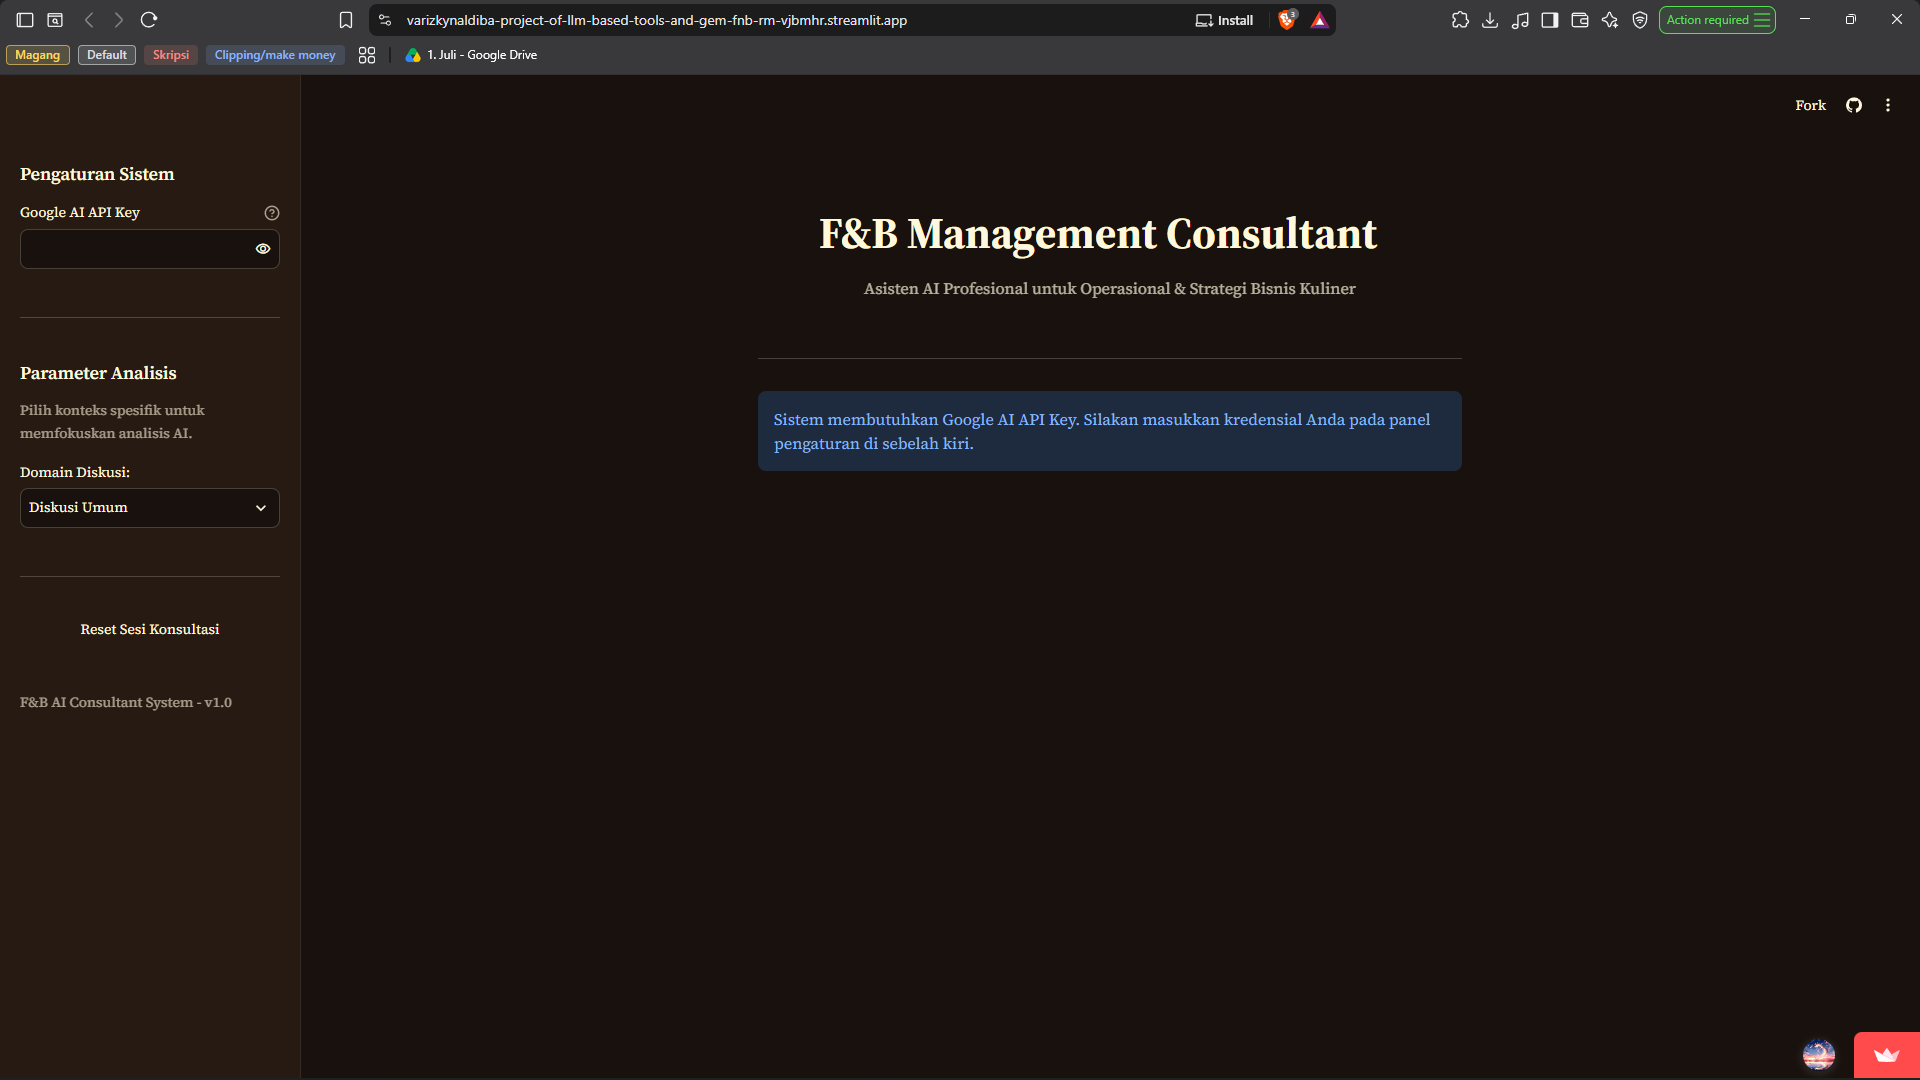
\includegraphics[width=\linewidth,height=3.6cm,keepaspectratio]{src/projects/09-ai-restaurant-advisory/assets/fnb-consultant-live.png}
      \end{tcolorbox}
      \vspace{2pt}
      \centering
      {\scriptsize \href{https://varizkynaldiba-project-of-llm-based-tools-and-gem-fnb-rm-vjbmhr.streamlit.app/}{\color{brandBlue}\textbf{\underline{[Live App: Streamlit F\&B Consultant $\nearrow$]}}}}
    \end{column}
    \begin{column}{0.50\textwidth}
      {\scriptsize \color{brandBlue} \textbf{GENERATIVE AI DECISION SUPPORT SYSTEM}} \hfill {\tiny \color{brandSlate} Proyek 09 / 13} \par \vspace{1pt}
      {\large \bfseries \color{brandNavy} AI Restaurant Advisory} \par
      {\scriptsize \bfseries \color{brandDark} Peran: Applied AI \& Data Scientist} \par
      {\tiny \color{brandSlate} \textbf{Tech Stack:} Python, Google Gemini API, Streamlit, Prompt Engineering, Pandas} \par \vspace{4pt}
      
      {\scriptsize \color{brandDark}
      $\bullet$ \textbf{Konsultan Bisnis Kuliner Digital:} Mengintegrasikan LLM Google Gemini dengan skema prompt terstruktur bebas halusinasi untuk operasional RM Padang. \\
      $\bullet$ \textbf{Menu Engineering Matrix (BCG):} Mengklasifikasikan menu secara deterministik ke dalam kategori Stars, Plowhorses, Puzzles, dan Dogs. \\
      $\bullet$ \textbf{Audit Resep \& Fluktuasi Bahan:} Menghitung food cost, margin keuntungan, serta rekomendasi penyesuaian porsi terhadap musim bahan baku.
      }
    \end{column}
  \end{columns}
\end{frame}

% ==============================================================================
% SLIDE 16: PROYEK 10 - FRUIT CLASSIFICATION
% ==============================================================================
\begin{frame}{P10: Fruit Classification CV}{EKSTRAKSI HIBRIDA \& SVM}
  \begin{columns}[c]
    \begin{column}{0.48\textwidth}
      \begin{tcolorbox}[colback=white,colframe=brandBorder,arc=2mm,boxrule=0.6pt,boxsep=1pt,top=2pt,bottom=2pt,halign=center]
        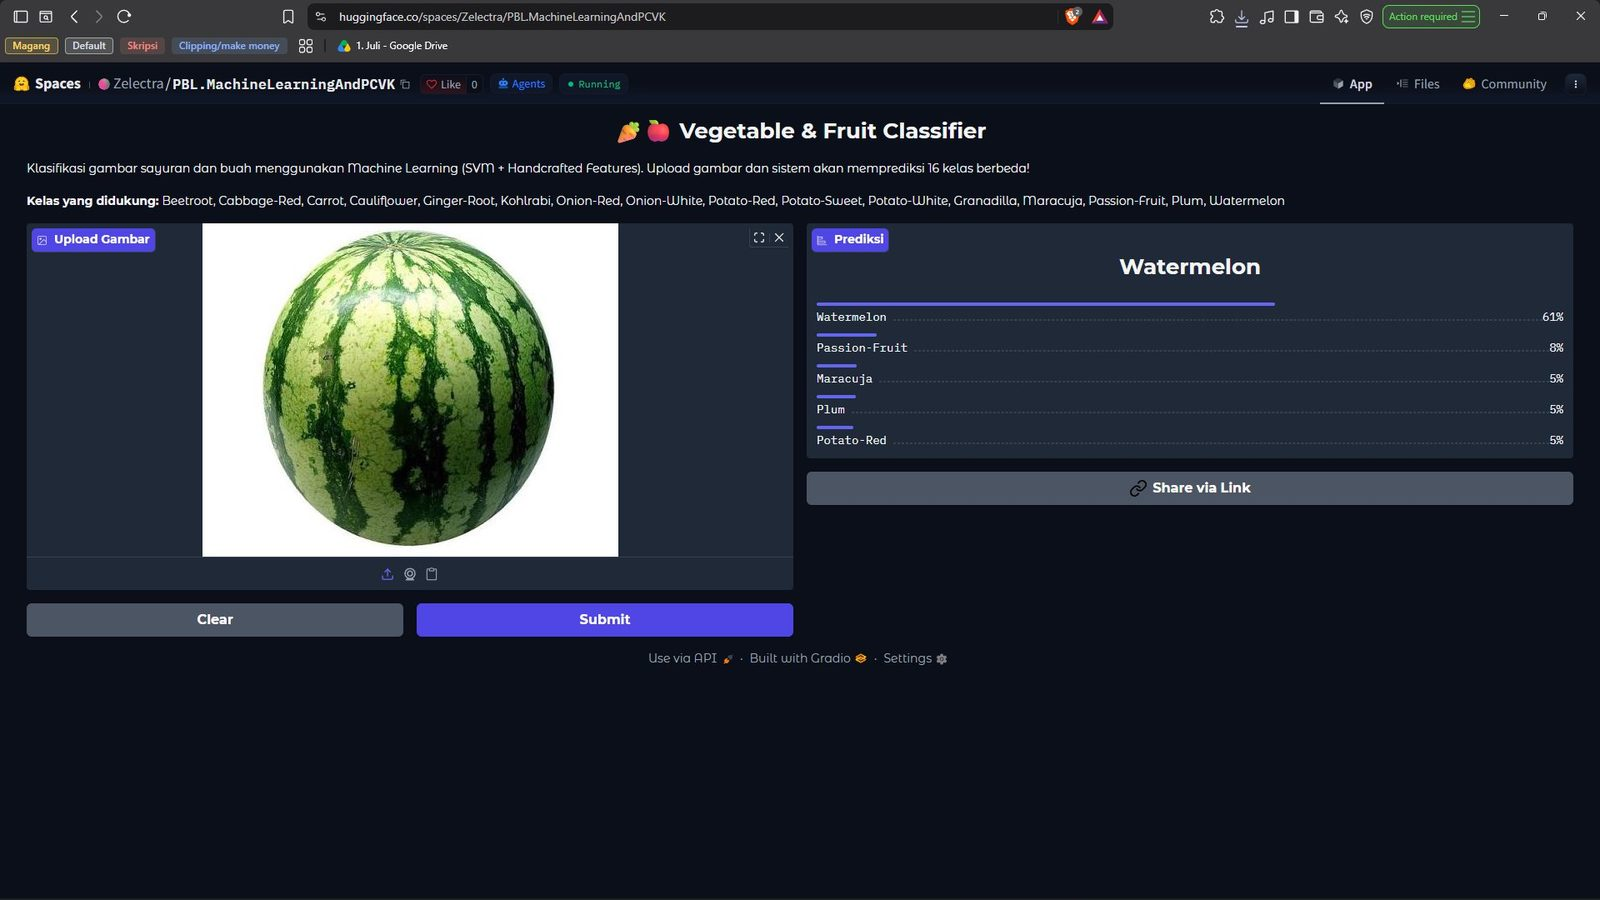
\includegraphics[width=\linewidth,height=3.6cm,keepaspectratio]{src/projects/10-fruit-classification/assets/fruit-classifier-live.jpg}
      \end{tcolorbox}
      \vspace{2pt}
      \centering
      {\scriptsize \href{https://huggingface.co/spaces/Zelectra/PBL.MachineLearningAndPCVK}{\color{brandBlue}\textbf{\underline{[HuggingFace: Live Classifier $\nearrow$]}}}}
    \end{column}
    \begin{column}{0.50\textwidth}
      {\scriptsize \color{brandBlue} \textbf{COMPUTER VISION PIPELINE \ $|$ \ 16 KELAS}} \hfill {\tiny \color{brandSlate} Proyek 10 / 13} \par \vspace{1pt}
      {\large \bfseries \color{brandNavy} Fruit Classification CV} \par
      {\scriptsize \bfseries \color{brandDark} Peran: Computer Vision \& ML Engineer} \par
      {\tiny \color{brandSlate} \textbf{Tech Stack:} Python, OpenCV, Scikit-Learn, GLCM, Wavelet 2D, HOG, SVM} \par \vspace{4pt}
      
      {\scriptsize \color{brandDark}
      $\bullet$ \textbf{Pengenalan 16 Varietas Tanpa GPU Berat:} Mengklasifikasikan buah dan sayuran secara akurat menggunakan kombinasi fitur handcrafted dan SVM. \\
      $\bullet$ \textbf{Ekstraksi Multi-Modal:} Menggabungkan matriks tekstur spasial GLCM, dekomposisi frekuensi Wavelet 2D, dan histogram orientasi gradien tepi HOG. \\
      $\bullet$ \textbf{Normalisasi Iluminasi CLAHE:} Mengoreksi gradien pencahayaan tidak merata agar inferensi stabil di aplikasi live HuggingFace.
      }
    \end{column}
  \end{columns}
\end{frame}

% ==============================================================================
% SLIDE 17: PROYEK 11 - SIMPRES
% ==============================================================================
\begin{frame}{P11: SIMPRES Polinema}{SISTEM PRESTASI \& PROMETHEE DSS}
  \begin{columns}[c]
    \begin{column}{0.48\textwidth}
      \begin{tcolorbox}[colback=white,colframe=brandBorder,arc=2mm,boxrule=0.6pt,boxsep=1pt,top=2pt,bottom=2pt,halign=center]
        
\includegraphics[width=\linewidth,height=3.6cm,keepaspectratio]{src/projects/11-simpres/assets/dashboard-simpres.jpg}
      \end{tcolorbox}
      \vspace{2pt}
      \centering
      {\scriptsize \href{https://github.com/VarizkyNaldiba/Prestasi-Mahasiswa-S4}{\color{brandBlue}\textbf{\underline{[GitHub: Prestasi-Mahasiswa-S4 $\nearrow$]}}}}
    \end{column}
    \begin{column}{0.50\textwidth}
      {\scriptsize \color{brandBlue} \textbf{SISTEM INFORMASI ENTERPRISE TI POLINEMA}} \hfill {\tiny \color{brandSlate} Proyek 11 / 13} \par \vspace{1pt}
      {\large \bfseries \color{brandNavy} SIMPRES Polinema} \par
      {\scriptsize \bfseries \color{brandDark} Peran: Full-Stack Developer \& Database Architect} \par
      {\tiny \color{brandSlate} \textbf{Tech Stack:} Laravel, PHP, MySQL, PROMETHEE DSS, Role-Based Access Control} \par \vspace{4pt}
      
      {\scriptsize \color{brandDark}
      $\bullet$ \textbf{Tata Kelola Prestasi Jurusan TI Polinema:} Mendigitalkan verifikasi capaian lomba mahasiswa, rekam jejak bimbingan dosen, dan sertifikasi. \\
      $\bullet$ \textbf{Algoritma SPK PROMETHEE:} Mencocokkan talenta dan keterampilan mahasiswa secara objektif dengan kriteria kompetisi nasional/internasional. \\
      $\bullet$ \textbf{Integritas Relasional ACID:} Desain skema basis data ternormalisasi tinggi yang menjamin konsistensi laporan akademik jurusan.
      }
    \end{column}
  \end{columns}
\end{frame}

% ==============================================================================
% SLIDE 18: PROYEK 12 - TATA TERTIB MAHASISWA
% ==============================================================================
\begin{frame}{P12: Tata Tertib Mahasiswa}{PENEGAKAN DISIPLIN POLINEMA}
  \begin{columns}[c]
    \begin{column}{0.48\textwidth}
      \begin{tcolorbox}[colback=white,colframe=brandBorder,arc=2mm,boxrule=0.6pt,boxsep=1pt,top=2pt,bottom=2pt,halign=center]
        
\includegraphics[width=\linewidth,height=3.6cm,keepaspectratio]{src/projects/12-tata-tertib-mahasiswa/assets/ui-tatib-full.png}
      \end{tcolorbox}
      \vspace{2pt}
      \centering
      {\scriptsize \href{https://github.com/VarizkyNaldiba/TataTertibMhs}{\color{brandBlue}\textbf{\underline{[GitHub: TataTertibMhs $\nearrow$]}}}}
    \end{column}
    \begin{column}{0.50\textwidth}
      {\scriptsize \color{brandBlue} \textbf{CAMPUS CODE-OF-CONDUCT PLATFORM}} \hfill {\tiny \color{brandSlate} Proyek 12 / 13} \par \vspace{1pt}
      {\large \bfseries \color{brandNavy} Sistem Tata Tertib Mahasiswa} \par
      {\scriptsize \bfseries \color{brandDark} Peran: Full-Stack Engineer \& UI/UX Designer} \par
      {\tiny \color{brandSlate} \textbf{Tech Stack:} Laravel, PHP, MySQL, Bootstrap 5, Figma Prototyping, Audit Logging} \par \vspace{4pt}
      
      {\scriptsize \color{brandDark}
      $\bullet$ \textbf{Transparansi Penegakan Disiplin Kampus:} Menggantikan pencatatan manual pelanggaran dengan alur kerja digital yang transparan dan akuntabel. \\
      $\bullet$ \textbf{Mekanisme Banding Bertingkat:} Alur sanggahan resmi dari mahasiswa dengan eskalasi persetujuan ke komisi disiplin jurusan dan dosen wali. \\
      $\bullet$ \textbf{Audit Trail Keamanan:} Pencatatan log terperinci terhadap setiap perubahan poin sanksi dan keputusan sanksi administratif.
      }
    \end{column}
  \end{columns}
\end{frame}

% ==============================================================================
% SLIDE 19: PROYEK 13 - SCHOOL SPATIAL GIS
% ==============================================================================
\begin{frame}{P13: School Spatial Distribution GIS}{KLASTERISASI SEKOLAH JATIM}
  \begin{columns}[c]
    \begin{column}{0.48\textwidth}
      \begin{tcolorbox}[colback=white,colframe=brandBorder,arc=2mm,boxrule=0.6pt,boxsep=1pt,top=2pt,bottom=2pt,halign=center]
        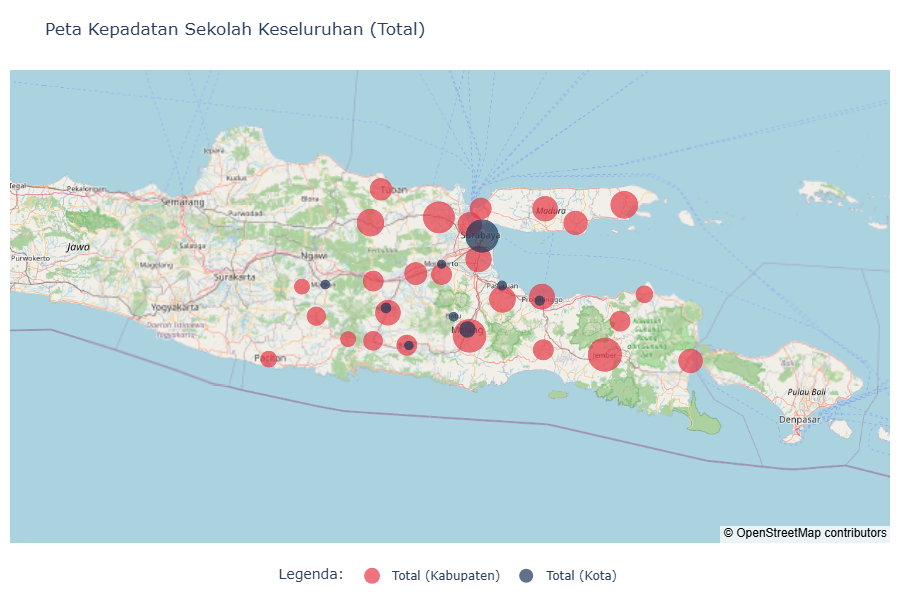
\includegraphics[width=\linewidth,height=3.6cm,keepaspectratio]{src/projects/13-school-spatial-gis/assets/peta-sebaran-total.png}
      \end{tcolorbox}
      \vspace{2pt}
      \centering
      {\scriptsize \href{https://github.com/VarizkyNaldiba/SchoolSpatial_on_EastJava}{\color{brandBlue}\textbf{\underline{[GitHub: SchoolSpatial\_on\_EastJava $\nearrow$]}}}}
    \end{column}
    \begin{column}{0.50\textwidth}
      {\scriptsize \color{brandBlue} \textbf{GEOSPATIAL ANALYTICS \& CLUSTERING}} \hfill {\tiny \color{brandSlate} Proyek 13 / 13} \par \vspace{1pt}
      {\large \bfseries \color{brandNavy} School Spatial GIS} \par
      {\scriptsize \bfseries \color{brandDark} Peran: Geospatial Analyst \& Python Developer} \par
      {\tiny \color{brandSlate} \textbf{Tech Stack:} Python, Folium GIS, GeoJSON, Pandas, Scikit-Learn (K-Means), Matplotlib} \par \vspace{4pt}
      
      {\scriptsize \color{brandDark}
      $\bullet$ \textbf{Analisis Densitas Pendidikan:} Memetakan radius layanan dan titik blank spot sekolah menengah (SMA/SMK) di 38 kab/kota Jawa Timur. \\
      $\bullet$ \textbf{Klasterisasi K-Means Spasial:} Mengelompokkan daerah dengan kepadatan tinggi vs terisolir berdasarkan koordinat geospasial aktual. \\
      $\bullet$ \textbf{Peta Choropleth Interaktif:} Visualisasi dinamis berbasis browser untuk analisis disparitas kualitas akses antarwilayah.
      }
    \end{column}
  \end{columns}
\end{frame}

% ==============================================================================
% SLIDE 20: METODOLOGI REKAYASA
% ==============================================================================
\begin{frame}{Metodologi \& Alur Kerja Rekayasa}{POLA REKAYASA SISTEM 3 TAHAP}
  \begin{columns}[t]
    \begin{column}{0.32\textwidth}
      \begin{tcolorbox}[colback=brandCardBg,colframe=brandBorder,arc=2mm,boxrule=0.6pt,boxsep=2pt,top=3pt,bottom=3pt,title={\footnotesize \bfseries \color{brandNavy} 01. Sensing \& Kalibrasi}]
        {\scriptsize \color{brandDark}
        $\bullet$ Akuisisi sinyal analog probe air (pH, kekeruhan, DO). \\
        $\bullet$ Kompensasi temperatur otomatis (probe DS18B20 seketika). \\
        $\bullet$ Kalibrasi kurva polinomial mengoreksi deviasi sensor. \\
        $\bullet$ Ring buffer flash lokal menjamin zero data loss.
        }
      \end{tcolorbox}
    \end{column}

    \begin{column}{0.32\textwidth}
      \begin{tcolorbox}[colback=brandCardBg,colframe=brandBorder,arc=2mm,boxrule=0.6pt,boxsep=2pt,top=3pt,bottom=3pt,title={\footnotesize \bfseries \color{brandNavy} 02. Preprocessing \& ML}]
        {\scriptsize \color{brandDark}
        $\bullet$ Pembersihan derau waktu dan rekayasa fitur harmonik. \\
        $\bullet$ Ekstraksi fitur visual spasial (MCNN, GLCM, Wavelet, HOG). \\
        $\bullet$ Pelatihan model prediktif (LSTM panen, Boosting cuaca). \\
        $\bullet$ Validasi metrik objektif (MAE, MSE, skor Kaggle).
        }
      \end{tcolorbox}
    \end{column}

    \begin{column}{0.32\textwidth}
      \begin{tcolorbox}[colback=brandCardBg,colframe=brandBorder,arc=2mm,boxrule=0.6pt,boxsep=2pt,top=3pt,bottom=3pt,title={\footnotesize \bfseries \color{brandNavy} 03. Deploy \& SPK}]
        {\scriptsize \color{brandDark}
        $\bullet$ Sinkronisasi data real-time ke datastore noSQL/SQL. \\
        $\bullet$ Perenderan lapisan spasial GeoJSON di web browser. \\
        $\bullet$ Algoritma penunjang keputusan (BCG matrix, PROMETHEE DSS). \\
        $\bullet$ Deploy cloud Vercel, HuggingFace Spaces \& Streamlit.
        }
      \end{tcolorbox}
    \end{column}
  \end{columns}
\end{frame}

% ==============================================================================
% SLIDE 21: DAMPAK & ANGKA PENCAPAIAN
% ==============================================================================
\begin{frame}{Dampak \& Angka Pencapaian Kunci}{METRIK REKAYASA \& CAPAIAN}
  \begin{columns}[t]
    \begin{column}{0.24\textwidth}
      \begin{tcolorbox}[colback=brandCardBg,colframe=brandBorder,arc=2mm,boxrule=0.6pt,halign=center,boxsep=3pt,top=5pt,bottom=5pt]
        {\LARGE \bfseries \color{brandNavy} 13} \par \vspace{2pt}
        {\scriptsize \bfseries \color{brandBlue} Sistem Rekayasa} \par \vspace{2pt}
        {\tiny \color{brandSlate} Solusi hulu-ke-hilir IoT, ML, WebGIS \& Enterprise.}
      \end{tcolorbox}
    \end{column}

    \begin{column}{0.24\textwidth}
      \begin{tcolorbox}[colback=brandCardBg,colframe=brandBorder,arc=2mm,boxrule=0.6pt,halign=center,boxsep=3pt,top=5pt,bottom=5pt]
        {\LARGE \bfseries \color{brandNavy} 94.310} \par \vspace{2pt}
        {\scriptsize \bfseries \color{brandBlue} Skor Akurasi Kaggle} \par \vspace{2pt}
        {\tiny \color{brandSlate} Peringkat 18 dari 82 tim nasional di Intelecta Cup.}
      \end{tcolorbox}
    \end{column}

    \begin{column}{0.24\textwidth}
      \begin{tcolorbox}[colback=amberBadgeBg,colframe=brandBorder,arc=2mm,boxrule=0.6pt,halign=center,boxsep=3pt,top=5pt,bottom=5pt]
        {\large \bfseries \color{amberBadgeText} Harapan 2} \par \vspace{2pt}
        {\scriptsize \bfseries \color{amberBadgeText} LKTI TFS 2026} \par \vspace{2pt}
        {\tiny \color{amberBadgeText} SK Direktur Polinema No. 27881/PL2.3/KM/2026.}
      \end{tcolorbox}
    \end{column}

    \begin{column}{0.24\textwidth}
      \begin{tcolorbox}[colback=brandCardBg,colframe=brandBorder,arc=2mm,boxrule=0.6pt,halign=center,boxsep=3pt,top=5pt,bottom=5pt]
        {\LARGE \bfseries \color{brandNavy} 0\%} \par \vspace{2pt}
        {\scriptsize \bfseries \color{brandBlue} Data Loss Buffer} \par \vspace{2pt}
        {\tiny \color{brandSlate} Failover flash memory ESP32 saat offline.}
      \end{tcolorbox}
    \end{column}
  \end{columns}
\end{frame}

% ==============================================================================
% SLIDE 22: MEDIA DIGITAL & KREATIF
% ==============================================================================
\begin{frame}{Divisi Media Digital \& Kreatif}{MEDIA DIGITAL \& KREATIF}
  \begin{columns}[t]
    \begin{column}{0.48\textwidth}
      \begin{tcolorbox}[colback=brandCardBg,colframe=brandBorder,arc=2mm,boxrule=0.6pt,boxsep=2pt,top=4pt,bottom=4pt,title={\footnotesize \bfseries \color{brandNavy} Saluran TikTok: @oryzasatirva}]
        {\scriptsize \color{brandDark}
        $\bullet$ \textbf{Fokus Konten:} Video pendek motion graphics, analisis taktis game, dan ritme pacing editorial berdurasi ringkas. \\
        $\bullet$ \textbf{Optimasi Retensi Audiens:} Menganalisis grafik drop-off penonton di detik-detik awal untuk memaksimalkan retensi algoritma. \\
        $\bullet$ \textbf{Aplikasi dalam Rekayasa:} Keterampilan menyampaikan gagasan teknis yang padat dan menarik secara visual kepada publik luas.
        } \par \vspace{4pt}
        {\scriptsize \href{https://www.tiktok.com/@oryzasatirva}{\color{brandBlue}\textbf{\underline{[TikTok: @oryzasatirva $\nearrow$]}}}}
      \end{tcolorbox}
    \end{column}

    \begin{column}{0.48\textwidth}
      \begin{tcolorbox}[colback=brandCardBg,colframe=brandBorder,arc=2mm,boxrule=0.6pt,boxsep=2pt,top=4pt,bottom=4pt,title={\footnotesize \bfseries \color{brandNavy} Saluran Bilibili: Space 1416802109}]
        {\scriptsize \color{brandDark}
        $\bullet$ \textbf{Fokus Konten:} Publikasi dokumentasi jangka panjang beresolusi tinggi dan panduan komprehensif mekanik taktis. \\
        $\bullet$ \textbf{Struktur Narasi:} Penyusunan bab breakdown analitis yang terstruktur bagi audiens komunitas dengan retensi tinggi. \\
        $\bullet$ \textbf{Kualitas Audio-Visual:} Penataan audio balancing, grading warna, dan kejelasan alur demonstrasi antarmuka.
        } \par \vspace{4pt}
        {\scriptsize \href{https://www.bilibili.tv/id/space/1416802109}{\color{brandBlue}\textbf{\underline{[Bilibili: Space 1416802109 $\nearrow$]}}}}
      \end{tcolorbox}
    \end{column}
  \end{columns}
\end{frame}

% ==============================================================================
% SLIDE 23: KONTAK & QR CODE
% ==============================================================================
\begin{frame}{Kontak Resmi \& Akses Portofolio}{KOMUNIKASI \& VERIFIKASI BERKAS}
  \begin{columns}[c]
    \begin{column}{0.62\textwidth}
      {\large \bfseries \color{brandNavy} Mari Berkolaborasi!} \par
      {\scriptsize \color{brandSlate} Terbuka untuk kesempatan rekayasa perangkat lunak, kolaborasi AI, dan telemetri IoT.} \par \vspace{8pt}
      
      \begin{tcolorbox}[colback=brandCardBg,colframe=brandBorder,arc=2mm,boxrule=0.6pt,boxsep=3pt,top=4pt,bottom=4pt]
        {\small \color{brandDark}
        $\bullet$ \textbf{Email Resmi:} \href{mailto:varizkynr@gmail.com}{\color{brandBlue}\textbf{varizkynr@gmail.com}} \\ \vspace{2pt}
        $\bullet$ \textbf{LinkedIn:} \href{https://www.linkedin.com/in/varizkynaldiba/}{\color{brandBlue}\textbf{linkedin.com/in/varizkynaldiba}} \\ \vspace{2pt}
        $\bullet$ \textbf{GitHub:} \href{https://github.com/VarizkyNaldiba}{\color{brandBlue}\textbf{github.com/VarizkyNaldiba}} \\ \vspace{2pt}
        $\bullet$ \textbf{Website:} \href{https://myprofile-nine-sigma.vercel.app/}{\color{brandBlue}\textbf{myprofile-nine-sigma.vercel.app}}
        }
      \end{tcolorbox}
      \vspace{4pt}
      {\scriptsize \color{brandSlate} Berkas resmi terverifikasi: \textbf{CV Dossier (PDF)} dan \textbf{Portofolio Deck (PDF)}.}
    \end{column}

    \begin{column}{0.34\textwidth}
      \begin{tcolorbox}[colback=white,colframe=brandBorder,arc=3mm,boxrule=0.8pt,halign=center,boxsep=3pt,top=4pt,bottom=4pt]
        
\includegraphics[width=0.75\linewidth,keepaspectratio]{public/portfolio-qr.png} \par \vspace{3pt}
        {\tiny \bfseries \color{brandNavy} Pindai QR untuk Akses Web} \par
        {\tiny \color{brandBlue} \href{https://myprofile-nine-sigma.vercel.app/}{myprofile-nine-sigma.vercel.app}}
      \end{tcolorbox}
    \end{column}
  \end{columns}
\end{frame}

\end{document}
